%%%%%%%%%%%%%%%%%%%%%%%%%%%%%%%%%
% 6CCS3PRJ Final Year Individual Project Report
% luke.day@kcl.ac.uk
%%%%%%%%%%%%%%%%%%%%%%%%%%%%%%%%%
\documentclass[11pt]{informatics-report}
\usepackage{color}
\usepackage[square,comma,numbers]{natbib}
% Required for [noitemsep] to work
\usepackage{enumitem}

% Other Forest-Flow packages
\usepackage{amsmath,amssymb,amsthm}
% Custom commands
\newcommand{\R}{\mathbb{R}}
\newcommand{\E}{\mathbb{E}}
\newcommand{\Prob}{\mathbb{P}}
\newcommand{\given}{\mid}
\usepackage{algorithm}
\usepackage{algpseudocode}
\usepackage{booktabs}
\usepackage{graphicx}
\graphicspath{{figures/}{../results/sweep_plots/}}
\usepackage{xcolor}
\usepackage{microtype}
\usepackage{tabularx}
\usepackage{array}
\usepackage{listings}%References
\lstdefinestyle{codeinline}{%
  basicstyle=\ttfamily,
  breaklines=true,
  columns=fullflexible,
}
\newcommand{\code}[1]{\lstinline[style=codeinline]!#1!}
% TikZ for architecture diagrams
\usepackage{tikz}
\usetikzlibrary{shapes.geometric,arrows.meta,positioning,fit,backgrounds,calc}
% Pandoc-compatible tight list (removes extra spacing in itemize/enumerate)
\providecommand{\tightlist}{%
  \setlength{\itemsep}{0pt}\setlength{\parskip}{0pt}}
%%%%%%%%%%%%%%%%%%%%%%%%%%%%%%%%%
% Front Matter - project title, name, supervisor name and date
%%%%%%%%%%%%%%%%%%%%%%%%%%%%%%%%%
\title{Synthetic ICU Trajectory Generation\\\vspace{0.2cm}via Heterogeneous Tree-Based Flow Matching}
\author{Lian Matsuo\\Programme of Study: Artificial Intelligence}
\studentID{K23060243}
\supervisor{David Watson}

\date{\today}

\abstractFile{FrontMatter/abstract.tex}
\ackFile{FrontMatter/acknowledgements.tex} %Remove line if you do not want acknowledgements

\begin{document}
\setlength{\emergencystretch}{3em}
\createFrontMatter
\onehalfspacing
\tableofcontents
\doublespacing

%%%%%%%%%%%%%%%%%%%%%%%%%%%%%%%%%
% Report Content
%%%%%%%%%%%%%%%%%%%%%%%%%%%%%%%%%
% You can write each chapter directly here or in a separate .tex file and use the include command.

\chapter{Introduction}

Healthcare data is difficult to share and model reliably at scale. Electronic Health Records (EHRs) combine mixed numerical and categorical variables, sparse and irregular dependencies, long-tailed outcomes, and domain rules that must be respected. Data-governance constraints under frameworks such as UK GDPR and the Data Protection Act 2018 further restrict access \cite{dataProtectionAct2018,icoResearchSafeguards}, while rare diseases and minority subpopulations create severe data scarcity and class imbalance. These weaknesses in real-world data availability and coverage are a core reason synthetic data generation is actively studied in healthcare.

Synthetic tabular generation can mitigate privacy and scarcity constraints, but common families still face limitations on mixed-type clinical data. GANs can underrepresent rare patterns, VAEs can oversmooth heterogeneous structure, and neural diffusion models often demand higher compute while requiring careful handling of categorical constraints.

Recent tree-based flow-matching work, especially ForestFlow \cite{jolicoeur2023forest} and HS3F \cite{akazan2024hs3f}, shows that gradient-boosted trees can approximate flow fields effectively for mixed-type tabular synthesis. This is directly relevant to ICU trajectories because tree partitions better match tabular heterogeneity and enable CPU-feasible training.

This project applies tree-based flow matching to sequential ICU patient trajectories derived from the MIMIC-III clinical database \cite{johnson2016mimic}. Unlike prior work that evaluates ForestFlow and HS3F on static, single-row tabular benchmarks, this project extends the approach to an autoregressive setting: a two-stage architecture where an independent and identically distributed (IID) hour-0 model generates initial patient states and a conditional model generates subsequent hourly transitions given lagged dynamics and static covariates. Two model backbones are implemented and compared: ForestFlow (all-continuous flow) and HS3F (heterogeneous sequential generation with separate continuous and categorical heads).

The objective is to investigate whether tree-based flow matching can produce synthetic ICU trajectories with useful fidelity, downstream utility, and privacy diagnostics while training efficiently on CPUs. The focus is technical feasibility and limitation-mapping rather than deployment claims.

Evaluation follows a multi-axis protocol: (1) \emph{fidelity} via Kolmogorov--Smirnov statistics, correlation preservation, and clinical range violation rates; (2) \emph{utility} via multi-task Train-on-Synthetic, Test-on-Real (TSTR) evaluation covering patient-level mortality prediction and ICU length-of-stay (LOS) prediction; and (3) \emph{privacy} via Distance-to-Closest-Record diagnostics and overfitting-based membership inference attacks (DOMIAS-style).

%==============================================================================
\section{Research Claim}
%==============================================================================

\noindent This dissertation argues that tree-based flow matching, originally formulated for static tabular data, can be adapted to sequential ICU trajectory synthesis on MIMIC-III through a two-stage autoregressive factorisation. Results from the sweep and matched backbone comparisons indicate technical feasibility: the generated data retains a measurable predictive signal and avoids exact-record copying in DCR checks. However, those same results also show practical limitations, particularly weak minority-class utility and high clinical range violations, so operational release readiness is not established.

%==============================================================================
\section{Aim and Objectives}
%==============================================================================

\paragraph{Aim:}
The aim of this project is to develop and evaluate a tree-based flow-matching framework for synthesising sequential ICU patient trajectories from the MIMIC-III clinical database \cite{johnson2016mimic}. The project assesses whether this approach can preserve useful structure across fidelity, downstream utility, privacy diagnostics, and computational efficiency in a reproducible research setting.

\paragraph{Objectives:}
This aim is operationalised through four concrete objectives:

\begin{description}[leftmargin=0cm,labelsep=0.6em]
    \item[Domain adaptation:] Extend ForestFlow \cite{jolicoeur2023forest} and HS3F \cite{akazan2024hs3f}, tree-based flow-matching models originally evaluated on static tabular benchmarks, to sequential clinical data via an autoregressive two-stage architecture comprising an IID hour-0 model for initial patient states and a conditional transition model for subsequent hourly dynamics.
    \item[Backbone implementation and comparison:] Implement both ForestFlow and HS3F within a unified training and evaluation interface so they can be compared under \textbf{identical} MIMIC preparation, data budgets, and evaluation code; the systematic hyperparameter grid (see below) is used to \textbf{map HS3F} over $(n_t, n_{\text{noise}})$, while the head-to-head evidence plan for all-continuous versus heterogeneous routing is a \textbf{pre-specified matched cell} (with CTGAN as a non-autoregressive reference), not a full per-cell multi-backbone matrix.
    \item[Multi-axis evaluation framework:] Develop a reproducible evaluation stack covering (i) distributional fidelity via Kolmogorov--Smirnov statistics, correlation preservation, and clinical range violation rates; (ii) downstream utility via multi-task Train-on-Synthetic, Test-on-Real (TSTR) evaluation covering patient-level mortality prediction and ICU length-of-stay (LOS) prediction; and (iii) privacy risk via Distance-to-Closest-Record diagnostics and DOMIAS-style membership inference attacks \cite{breugel2023domias}.
    \item[Systematic hyperparameter investigation:] Evaluate the effect of key flow-matching hyperparameters ($n_t$, $n_{\text{noise}}$) on synthetic data quality, utility, and computational cost via a reproducible, resumable grid sweep.
\end{description}

\paragraph{Research questions:}
The objectives above are evaluated through the following specific research questions:

\begin{description}[leftmargin=0cm,labelsep=0.6em]
    \item[Feasibility:] Can tree-based flow matching, originally evaluated on static tabular benchmarks, be extended to generate realistic sequential ICU trajectories via autoregressive conditioning?
    \item[Heterogeneous features (matched backbones):] At a fixed, shared hyperparameter cell with identical MIMIC cohort, training budget, and trajectory seeds, how do fidelity- and utility-relevant metrics compare between HS3F (explicit continuous/categorical heads) and ForestFlow (all-continuous flow) on the same mixed-type autoregressive tables? (The $8 \times 8$ sweep in this thesis \textbf{characterises HS3F} over $(n_t, n_{\text{noise}})$; it is not, and is not presented as, a grid in which every cell reruns all backbones. Evidence for the backbone question is the matched design in section~\ref{sec:backbone-comparison}.)
    \item[Utility and privacy:] Do synthetic trajectories preserve sufficient downstream predictive signal (TSTR) while maintaining acceptable privacy-risk indicators under proximity-based and attack-based diagnostics?
\end{description}

Throughout the report, a central distinction is maintained between \emph{research feasibility} and \emph{practical adequacy}: a configuration may generate coherent trajectories and transfer a predictive signal while still falling short of release or operational standards.

Although this project does not propose new generative algorithms, it contributes an \textbf{application-level integration} of existing tree-based flow-matching methods into a new domain (sequential clinical data) and a new problem structure (autoregressive trajectory generation).
The contribution lies in the system design, the multi-axis evaluation framework, and the empirical investigation of how these methods behave when adapted from static benchmarks to the challenges of temporal, mixed-type ICU data.

\chapter{Background}

\section{Motivation}
\subsection{Problem with Current Approaches}
Synthetic tabular data generation is motivated by three core pressures: privacy, data scarcity, and the need for high-fidelity statistical structure in domains such as healthcare where data is high-dimensional, mixed-type, and heavily constrained. Benchmarking studies and scoping reviews of synthetic EHR generation consistently demonstrate that tabular data poses a uniquely difficult challenge: it contains heterogeneous feature types, nonlinear dependencies, rare-event structure, and logical or physiological rules that must be respected to avoid producing implausible records \cite{yan2022benchmarking,kaabachi2025scoping}. Models must therefore capture both the statistical distribution and the structural constraints of the data.

\subsubsection{Limitations of Current Generative Approaches}

Across the literature, traditional generative paradigms struggle with at least one of the following:
\begin{enumerate}
    \item \textbf{GAN-based models} (e.g., CTAB-GAN \cite{zhao2021ctabgan}, medGAN \cite{choi2017medgan}):
    GANs excel at image-like continuous domains but degrade in tabular settings because mixed categorical--numerical variables break the smoothness assumptions of adversarial training. They are also prone to mode collapse, leading to missing rare patterns---critical in healthcare datasets. Benchmarking studies show GAN-based EHR models consistently failing on minority disease codes, rare laboratory patterns, and sparse temporal events \cite{yan2022benchmarking}.

    \item \textbf{Diffusion models} (e.g., TabDDPM \cite{kotelnikov2023tabddpm}, TabDiff \cite{shi2025tabdiff}):
    Diffusion improves training stability but still struggles to enforce structured constraints (e.g., mutually exclusive diagnosis codes, age--procedure consistency). Jolicoeur-Martineau et al.\ \cite{jolicoeur2023forest} argue that naïvely diffusing mixed-type features introduces discontinuities and destroys interpretability unless additional structure is imposed.

    \item \textbf{LLMs as generators}:
    While LLMs are powerful generative models \cite{borisov2023great,wang2022promptehr}, they are not naturally statistical samplers. Without ground-truth marginals or explicit constraints, they can hallucinate records that appear plausible but fail distributional tests, break medical validity rules, or exhibit memorisation risk---a risk noted in evaluations of transformer-based EHR generation \cite{yan2022benchmarking}.
\end{enumerate}

\subsection{Why Trees?}

The literature converges on a key theme: tabular data has structure that trees capture naturally, while neural generative models do not. This is the central motivation behind the ForestFlow family of methods \cite{jolicoeur2023forest,akazan2024hs3f} and several hybrid systems that use gradient-boosted trees as the generative backbone.

\begin{enumerate}
    \item \textbf{Trees partition the space into meaningful, homogeneous regions.}
    Tree ensembles (GBTs, Random Forests, XGBoost) split data recursively along informative feature thresholds. This has two consequences:
    \begin{enumerate}
        \item \emph{Locality}: each leaf corresponds to a region where data is homogeneous with respect to key interactions.
        \item \emph{Conditional modelling}: within a leaf, modelling the distribution is dramatically easier---categorical frequencies and numerical distributions become far more structured.
    \end{enumerate}
    Jolicoeur-Martineau et al.\ \cite{jolicoeur2023forest} exploit this by training boosted trees whose leaves encode low-dimensional conditional distributions used during flow or diffusion sampling. EHR data is multiscale and multimodal, with many modes corresponding to clinically meaningful subpopulations (e.g., diabetic patients with renal impairment) that trees isolate naturally \cite{yan2022benchmarking}.

    \item \textbf{Trees capture nonlinear interactions and rare-class structure.}
    Benchmarking studies show that many synthetic generators fail on minority-class fidelity and long-tail patterns \cite{yan2022benchmarking,kaabachi2025scoping}.
    Trees, however:
    \begin{itemize}
        \item create leaves dominated by small cohorts, preserving rare but real combinations;
        \item do not require smoothness assumptions;
        \item naturally handle categorical features without embedding instabilities.
    \end{itemize}
    This addresses the rare-disease problem, where GAN adversarial losses dominated by majority cases fail to reproduce minor diagnostic categories \cite{yan2022benchmarking}.
    Rare-class preservation is a central motivation for using trees in the healthcare domain.

    \item \textbf{Trees provide interpretability and explainable generative structure.}
    Diffusion models and GANs are largely black boxes.
    Tree partitions, by contrast, provide:
    \begin{itemize}
        \item transparent decision boundaries;
        \item interpretable splits that correspond to medical and business logic (e.g., ``if age $>$ 50 and BP $<$ threshold $\rightarrow$ leaf'');
        \item auditability of conditional distributions.
    \end{itemize}
    For regulated domains such as EHRs, this is essential: EHR synthesis requires mechanisms that can be audited for safety and plausibility \cite{kaabachi2025scoping}, a requirement that trees satisfy in a way neural generators do not.

    \item \textbf{Trees can be combined with flow or diffusion models to become fully generative.}
    Jolicoeur-Martineau et al.\ \cite{jolicoeur2023forest} introduce the key conceptual innovation: using tree-based function approximation within a flow-matching generative pipeline.
    Instead of learning vector fields across the entire mixed-type space with a neural network, the model uses XGBoost regressors at each discrete time level, where:
    \begin{itemize}
        \item feature interactions are captured by tree splits;
        \item categorical variables are handled via explicit classifier heads (HS3F \cite{akazan2024hs3f});
        \item numerical features are transported by continuous flows within locally homogeneous regions.
    \end{itemize}
    This combination addresses the core weaknesses of neural-only models on tabular data.

    \item \textbf{Trees encode constraints better than pure neural models.}
    Logical constraints---sex--pregnancy consistency, ICD code compatibility, physiological ranges---are difficult to learn implicitly from data.
    Trees help because:
    \begin{itemize}
        \item splits often correspond to implicit constraints (``pregnancy-related codes $\rightarrow$ female leaves only'');
        \item each leaf forms a coherent subpopulation, reducing the risk of constraint violations;
        \item constraint checking becomes local rather than global.
    \end{itemize}
\end{enumerate}

\subsection{The Healthcare Domain}

The healthcare domain was chosen for three compounding reasons:
\begin{itemize}
    \item \textbf{Constraint:} healthcare data is one of the most constrained data formats, due to acute concerns of privacy, scarcity, and complexity. Real patient records are difficult to share due to regulations such as HIPAA and GDPR \cite{dataProtectionAct2018}. Scarcity is common especially for rare conditions, meaning many clinical AI projects suffer from small sample sizes and extreme class imbalance.
    \item \textbf{Relevancy:} EHRs contain structured fields amounting to hundreds of variables, many of which are mixed-type (continuous vital signs, binary intervention flags, categorical diagnosis codes). Healthcare data also comes with logical and physiological constraints that must be preserved: patients coded as male cannot have a pregnancy diagnosis, laboratory values must remain within humanly plausible ranges, and procedure codes should align with diagnosis codes.
    \item \textbf{Impact:} there is an established and growing need for synthetic data in healthcare research to enable sharing and analysis without compromising patient privacy \cite{kaabachi2025scoping,yan2022benchmarking}. Synthetic data also offers a principled mechanism to address class imbalance in rare-event clinical prediction tasks.
\end{itemize}

\section{Literature Review}
\subsection[ForestFlow (Jolicoeur-Martineau et al., 2023)]{Review of \textit{Generating and Imputing Tabular Data via Diffusion and Flow-Based Gradient-Boosted Trees} (Jolicoeur-Martineau et al., 2023)}
\subsubsection{Problem Explored}
Jolicoeur-Martineau et al.\ (2023) investigate how to perform both synthetic data generation and missing-value imputation for tabular datasets using diffusion models and flow-matching, but with a key departure from prior work: instead of neural networks, they use gradient-boosted decision trees (GBTs) to approximate the score function or vector field required by these generative frameworks. Their motivation arises from the observation that traditional deep generative models---such as GANs, VAEs, or neural diffusion networks---struggle with mixed-type tabular data, discontinuous feature relationships, rare categories, and non-random missingness. Since tree-based models are more naturally adapted to these characteristics and do not assume smoothness, the authors reframe diffusion and flow-based generative modelling around GBTs to better capture tabular structure.

Past work on score-based generative models has overwhelmingly relied on neural networks, particularly for continuous domains like images. In the tabular case, these neural models often distort categorical distributions, fail to preserve joint dependencies, and require heavy computational resources. The authors position their work as a practical and more data-appropriate alternative.

\subsubsection{Proposed Method}
The proposed system, termed \textit{ForestDiffusion}, implements either a score-based diffusion model or a flow-matching model, but replaces neural score or vector-field approximators with gradient-boosted trees. In the diffusion formulation, the model assumes a forward noising process
\begin{equation}
    dx_t = f(t) x_t \, dt + g(t) \, dW_t,
\end{equation}
and trains a tree model to estimate the score
\begin{equation}
    s_\theta(x_t, t) \approx \nabla_x \log p_t(x_t).
\end{equation}
This score predictor is learned by regressing on the noise injected at time~$t$, following standard diffusion-model training principles \cite{song2021scoresde}. Sampling begins from a noise distribution and integrates the corresponding reverse-time SDE using the learned score model.

In the flow-matching variant, the method learns a time-dependent vector field
\begin{equation}
    v_\theta(x, t) \approx \frac{d x_t}{dt},
\end{equation}
which defines an ODE transporting samples from a simple reference distribution (e.g., Gaussian) to the target tabular distribution. Synthetic data are obtained by integrating this ODE across time.

Because GBTs operate directly in feature space, they naturally preserve discrete boundaries, handle heterogeneous feature types, and adapt well to irregular dependencies. The same model supports \textit{imputation}: given partially observed data, the diffusion or flow dynamics are conditioned on the known coordinates, and the missing entries are inferred through the generative process.

\subsubsection{Findings and Empirical Results}
The authors conduct extensive experiments on 27 real-world tabular datasets, evaluating both data generation and missing-value imputation across nine quantitative metrics. Their results show that tree-based diffusion and flow models are highly competitive with, and frequently outperform, neural generative models, especially on mixed-type datasets. The generated samples exhibit strong fidelity in marginals, correlations, multimodal patterns, and categorical distributions.

For imputation, the method performs comparably to state-of-the-art imputation techniques, despite functioning as a general-purpose generative model rather than a specialised imputation framework. A significant practical contribution is that the entire system can be trained efficiently using CPU parallelism, avoiding the need for GPU-heavy neural networks.

\subsubsection{Future Work and Limitations}
The authors note that categorical variables remain challenging to embed cleanly into continuous-time diffusion or flow processes, and suggest that improved treatment of categorical noise processes may enhance performance. The method also requires training multiple GBT models across time steps, which can be memory-intensive; future work may explore parameter sharing or sparse representations. Additional extensions include conditional tabular generation, temporal or relational tabular structures, and hybrid tree--neural approaches. While imputation performance is strong, specialised imputation models can still outperform it under extreme missingness, indicating room for improved conditional sampling.

\subsection{Review of \textit{Generating Tabular Data Using Heterogeneous Sequential Feature Forest Flow Matching} (Akazan et al., 2024)}

\subsubsection{Problem Explored}
Akazan et al.\ (2024) address a key limitation of ForestFlow: its treatment of all feature dimensions as continuous during flow matching. In real-world tabular datasets, categorical variables are discrete and cannot be meaningfully interpolated along a continuous flow path. Naively noising categorical columns with Gaussian noise and rounding at generation time degrades sample quality, particularly when the number of categories is large or the categorical distribution is highly skewed.

\subsubsection{Proposed Method}
The proposed method, Heterogeneous Sequential Feature Forest Flow (HS3F), decomposes the joint distribution over features into a product of conditionals, generating features one at a time in a fixed order:
\begin{equation}
p(\mathbf{x}) = \prod_{j=1}^{d} p(x_j \mid x_1, \ldots, x_{j-1}).
\end{equation}

For each feature $j$ in this sequence:
\begin{itemize}
    \item If $j$ is continuous: a flow-matching model (with XGBoost regressors) is trained and sampled, as in ForestFlow.
    \item If $j$ is categorical: an XGBoost multi-class classifier is trained and the class is sampled from the predicted distribution.
\end{itemize}

Each feature’s model is conditioned on all previously generated features, enabling the sequential process to capture inter-feature dependencies. The method retains the CPU-friendly, tree-based architecture of ForestFlow while properly handling discrete outputs.

\subsubsection{Findings and Empirical Results}
On standard tabular benchmarks, HS3F matches or outperforms ForestFlow on datasets with substantial categorical content, while maintaining comparable performance on purely continuous datasets. The sequential feature generation adds computational cost proportional to the number of features, but avoids the noise-then-round artefacts that degrade ForestFlow’s categorical fidelity.

\subsubsection{Relevance to This Project}
HS3F is directly relevant because ICU data from MIMIC-III contains a mixture of continuous vital signs, binary intervention flags, and categorical variables. The project implements both ForestFlow and HS3F as selectable backbones, allowing empirical comparison of the two approaches on clinical data where categorical fidelity is clinically meaningful (e.g., binary ventilation status, categorical diagnosis codes).

\subsection{MIMIC-III and the MIMIC-Extract Pipeline}

\subsubsection{Source Database}
MIMIC-III (Medical Information Mart for Intensive Care III) is a freely accessible critical care database comprising deidentified health data for over 40,000 ICU patients at Beth Israel Deaconess Medical Center \cite{johnson2016mimic}. It contains demographics, vital signs, laboratory measurements, medications, procedures, clinical notes, and outcome data, recorded at irregular intervals throughout each ICU stay.

\subsubsection{MIMIC-Extract Representation}
MIMIC-Extract \cite{wang2020mimicextract} provides a standardised pipeline that transforms the irregularly sampled MIMIC-III data into hourly feature matrices suitable for machine learning. The pipeline handles missing-value imputation, unit conversion, and outlier removal, producing a rectangular table where each row represents one patient-hour with a consistent feature set. This hourly representation is the canonical input to the autoregressive modelling pipeline in the current project.

\subsubsection{Relevance to This Project}
The choice of MIMIC-III via MIMIC-Extract provides a well-studied, high-dimensional, mixed-type clinical dataset with known properties and established benchmarks. It also imposes specific data-governance obligations (credentialing, data use agreement) that are addressed in the legal and ethical analysis of this report.

\subsection{Existing Synthetic Tabular and EHR Generators}

Several established generator families serve as reference points for this work. The project includes a CTGAN/CRGAN-style lower-bound baseline in the implemented evaluation pipeline, while broader architecture-parity comparisons across other generator families remain future work. Their methodological characteristics motivate the design choices in this project.

\subsubsection{GAN-Based Generators}
\begin{itemize}\tightlist
    \item \textbf{CTGAN} \cite{xu2019ctgan}: A conditional GAN for tabular data that uses mode-specific normalisation to handle multimodal continuous distributions and training-by-sampling to address class imbalance. CTGAN is widely used but is susceptible to mode collapse on high-dimensional mixed-type data.
    \item \textbf{TimeGAN} \cite{yoon2019timegan}: A GAN variant specifically designed for time-series data, combining an autoencoder with adversarial training in a learned embedding space. TimeGAN addresses temporal structure but requires GPU training and careful hyperparameter tuning.
\end{itemize}

\subsubsection{Diffusion and Score-Based Generators}
\begin{itemize}\tightlist
    \item \textbf{TabDDPM} \cite{kotelnikov2023tabddpm}: A denoising diffusion probabilistic model adapted for mixed-type tabular data, applying multinomial diffusion to categorical features and Gaussian diffusion to continuous features. TabDDPM demonstrated superiority over GAN/VAE alternatives on extensive benchmarks at ICML~2023 and is a leading neural baseline in tabular generation.
    \item \textbf{TabSyn} \cite{zhang2024tabsyn}: Combines a VAE-crafted latent space with score-based diffusion, achieving state-of-the-art results on mixed-type generation at ICLR~2024 (oral presentation) with 86\% reduction in column-wise distribution error and 67\% reduction in correlation error over prior methods.
    \item \textbf{STaSy} \cite{kim2023stasy}: A score-based tabular data synthesis method that applies score matching with self-paced learning to handle the heterogeneity of tabular features.
\end{itemize}

\subsubsection{Transformer-Based Generators}
\begin{itemize}\tightlist
    \item \textbf{GReaT} \cite{borisov2023great}: Uses fine-tuned large language models (GPT-2) to generate tabular data by serializing rows as text. Achieves competitive results on standard benchmarks without architectural modifications for tabular structure.
    \item \textbf{REaLTabFormer} \cite{solatorio2023realtabformer}: A two-stage transformer using an autoregressive GPT-2 model for parent tables and a sequence-to-sequence model for relational data, with a novel $Q_\delta$ overfitting detection statistic.
    \item \textbf{PromptEHR} \cite{wang2022promptehr}: Applies prompt learning to conditional EHR generation on MIMIC-III, formulating generation as text-to-text translation with support for longitudinal, cross-modal, and conditional generation.
\end{itemize}

\subsubsection{Toolkits and Ecosystems}
\begin{itemize}\tightlist
    \item \textbf{SDV ecosystem} \cite{sdvproject}: The Synthetic Data Vault provides a suite of tabular and sequential generators (including GaussianCopula, CTGAN, and PAR for sequential data) with integrated evaluation metrics. It represents the most accessible baseline ecosystem for synthetic tabular data.
\end{itemize}

The tree-based approach taken in this project is motivated by the observation that neural generators often require GPU resources, extensive hyperparameter tuning, and architectural customisation for mixed-type data, while tree ensembles provide strong inductive biases for tabular structure without these constraints.

\chapter{Requirements and Specification}

This chapter defines the functional and non-functional requirements for the synthetic ICU trajectory generation system, derived from the research objectives stated in Chapter~1. Requirements are prioritised using the MoSCoW method (Must, Should, Could, Won't) and linked to verification criteria used in later evaluation.

%==============================================================================
\section{Use Cases}
%==============================================================================

Synthetic ICU trajectory generation is a research-facing capability rather than a consumer product. Accordingly, the actors identified here are organisations and individuals engaged in clinical data science, machine-learning research, and healthcare data governance---the three communities for which synthetic EHR generators have the most documented practical value \cite{yan2022benchmarking,kaabachi2025scoping}.

\subsection{Actors}

\begin{description}
    \item[\textbf{Clinical Data Custodian (CDC).}] A data engineer or clinical informatics specialist at a hospital or research institute who holds a credentialed dataset (e.g.\ MIMIC-III) and wishes to derive a shareable synthetic analogue. This actor is primarily motivated by data-governance obligations---privacy regulations such as HIPAA and GDPR restrict direct sharing of raw patient records \cite{dataProtectionAct2018}. The CDC runs the training and generation pipeline and is responsible for evaluating the privacy properties of the synthetic output before any release.

    \item[\textbf{Downstream ML Researcher (MLR).}] A machine-learning researcher or data scientist who requires realistic ICU time-series data to develop, benchmark, or fine-tune clinical prediction models (e.g.\ mortality prediction, sepsis onset, ICU length-of-stay classifiers) but does not have direct access to a credentialed patient dataset. The MLR receives a synthetic cohort from the CDC and uses it as a training corpus \cite{yan2022benchmarking}.

    \item[\textbf{Privacy Auditor (PA).}] A member of an institutional review board, data governance committee, or responsible-disclosure team who must verify that a synthetic dataset does not memorise training-set individuals before it is approved for external release. The PA runs the privacy evaluation suite and interprets the resulting risk metrics against institutional thresholds \cite{kaabachi2025scoping,yao2025dcrdelusion}.
\end{description}

\subsection{Use Case 1: Privacy-Preserving Data Release}

\textbf{Actor:} Clinical Data Custodian (CDC). \\
\textbf{Goal:} Generate a synthetic ICU cohort that can be shared with external collaborators without disclosing real patient records.

\begin{enumerate}
    \item The CDC obtains credentialed MIMIC-III access and produces hourly ICU tables via a MIMIC-Extract style preprocessing pipeline.
    \item The CDC runs the data preparation scripts (\texttt{00\_prepare}, \texttt{01\_preprocess}) to build autoregressive training tables.
    \item The CDC fits the tabular preprocessor on the full dataset (\texttt{01b\_fit\_preprocessor}) to capture all categorical values and numeric ranges.
    \item The CDC trains the generative model (\texttt{02\_train\_model}) using the preferred backbone (ForestFlow or HS3F).
    \item The CDC generates a synthetic patient cohort (\texttt{03\_generate\_synthetic}) at the desired scale.
    \item The CDC runs the privacy evaluation suite and reviews DCR diagnostics and membership inference attack scores.
    \item If privacy risk is within acceptable thresholds, the synthetic cohort is packaged and shared with the MLR. Real patient tables are never distributed.
\end{enumerate}

\textbf{Success criterion:} DCR overfitting-protection score $\geq$ threshold; DOMIAS-style MIA ROC-AUC near chance level; no exact-match records in synthetic output.

\subsection{Use Case 2: Synthetic-Data-Augmented Model Development}

\textbf{Actor:} Downstream ML Researcher (MLR). \\
\textbf{Goal:} Train and evaluate clinical prediction models using a synthetic cohort as a substitute or augmentation for real ICU data.

\begin{enumerate}
    \item The MLR receives a synthetic ICU trajectory CSV from the CDC (Use Case~1).
    \item The MLR trains a downstream clinical classifier (e.g.\ mortality predictor, LOS classifier) on the synthetic training split.
    \item The MLR evaluates the trained classifier on a held-out \emph{real} test set (TSTR protocol \cite{esteban2018rcgan}).
    \item The MLR compares TSTR performance to a real-data baseline (TRTR) to assess the utility of the synthetic cohort.
    \item If utility is insufficient, the MLR requests a regeneration from the CDC with adjusted hyperparameters or a larger synthetic cohort.
\end{enumerate}

\textbf{Success criterion:} Synthetic-trained classifier achieves ROC-AUC within an acceptable gap of the real-trained baseline; F1 scores indicate minority-class retention.

\subsection{Use Case 3: Privacy Audit Prior to Data Release}

\textbf{Actor:} Privacy Auditor (PA). \\
\textbf{Goal:} Independently verify that the synthetic dataset approved by the CDC does not expose training-set individuals before external release is approved.

\begin{enumerate}
    \item The PA receives the synthetic cohort and the evaluation artifacts (sweep log, privacy metrics) from the CDC.
    \item The PA re-runs the privacy evaluation module (\texttt{privacy\_metrics.py}) on the synthetic cohort against the held-out real data.
    \item The PA inspects DCR distributions, baseline and overfitting protection scores, and MIA ROC-AUC.
    \item The PA cross-references findings against the DCR-delusion literature \cite{yao2025dcrdelusion}---recognising that proximity metrics alone are not sufficient anonymity evidence---and supplements with DOMIAS-style attack results.
    \item The PA issues a release recommendation, with caveats on subgroup populations or features where risk remains elevated.
\end{enumerate}

\textbf{Success criterion:} MIA attacker advantage is near zero; no individual synthetic record matches a real training record exactly; privacy report is documented alongside the synthetic dataset.

%==============================================================================
\section{Functional Requirements}
%==============================================================================

\begin{table}[htbp]
\centering
\small
\setlength{\tabcolsep}{3pt}
\begin{tabularx}{\textwidth}{@{}ll>{\raggedright\arraybackslash}Xl@{}}
\toprule
\textbf{ID} & \textbf{Priority} & \textbf{Requirement} & \textbf{Verification} \\
\midrule
FR1 & Must & The system must preprocess MIMIC-III hourly ICU tables into an autoregressive format with lag-1 features, separating static and dynamic columns. & Unit tests; output CSV inspection \\
\midrule
FR2 & Must & The system must fit a tabular preprocessor on the full dataset via streaming to capture all categorical values and numeric ranges. & Preprocessor artifact; inverse-transform round-trip \\
\midrule
FR3 & Must & The system must train a conditional generative model (ForestFlow or HS3F) on the autoregressive data, learning $p(\mathbf{x}_t \mid \mathbf{x}_{t-1}, \mathbf{s})$. & Model artifact; unit tests \\
\midrule
FR4 & Must & The system must generate synthetic patient trajectories by autoregressively sampling from the trained model. & Output CSV; row count \\
\midrule
FR5 & Must & The system must evaluate synthetic data quality via KS statistics, correlation preservation, and clinical range violation rates. & Quality metrics output \\
\midrule
FR6 & Must & The system must evaluate downstream utility via multi-task patient-level TSTR covering mortality and ICU length-of-stay prediction. & TSTR metrics in sweep CSV \\
\midrule
FR7 & Should & The system should train an IID hour-0 model for fully synthetic generation without requiring real initial conditions. & Hour-0 model artifact \\
\midrule
FR8 & Should & The system should evaluate privacy risk via DCR diagnostics and membership inference attacks. & Privacy metrics output \\
\midrule
FR9 & Should & The system should support both ForestFlow and HS3F backbones via a unified interface with backbone selection. & CLI flag; unit tests \\
\midrule
FR10 & Could & The system could provide visualisation of sweep results across hyperparameter configurations. & Plot output files \\
\bottomrule
\end{tabularx}
\caption{Functional requirements with MoSCoW priorities.}
\label{tab:func-req}
\end{table}

%==============================================================================
\section{Non-Functional Requirements}
%==============================================================================

\begin{table}[htbp]
\centering
\small
\setlength{\tabcolsep}{3pt}
\begin{tabularx}{\textwidth}{@{}ll>{\raggedright\arraybackslash}Xl@{}}
\toprule
\textbf{ID} & \textbf{Priority} & \textbf{Requirement} & \textbf{Verification} \\
\midrule
NFR1 & Must & The system must be reproducible: deterministic seeds, explicit artifact paths, and canonical CSV schemas. & Repeated runs; seed logging \\
\midrule
NFR2 & Must & The system must train on CPU without requiring GPU resources. & Successful training on CPU-only machine \\
\midrule
NFR3 & Must & The system must not commit or expose real patient data in version-controlled artifacts. & \texttt{.gitignore} rules; repository inspection \\
\midrule
NFR4 & Should & The system should handle datasets with up to 2 million rows without exceeding available memory. & Memory-efficient data iterator \\
\midrule
NFR5 & Should & The hyperparameter sweep should be resumable, skipping previously completed configurations. & Sweep rerun behaviour \\
\midrule
NFR6 & Should & The system should include a unit test suite with $>$50 tests covering core modules. & \texttt{pytest} output \\
\midrule
NFR7 & Could & The system could cache transformed data matrices to avoid redundant preprocessing across sweep runs. & Cache hit/miss logging \\
\bottomrule
\end{tabularx}
\caption{Non-functional requirements with MoSCoW priorities.}
\label{tab:nonfunc-req}
\end{table}

%==============================================================================
\section{Specification}
%==============================================================================

\subsection{Data Specification}

\begin{itemize}\tightlist
    \item \textbf{Input}: MIMIC-III hourly ICU tables produced by a MIMIC-Extract style pipeline, containing mixed-type features (continuous vital signs, binary intervention flags, categorical codes) and static demographics.
    \item \textbf{Autoregressive format}: Each row represents one patient-hour, with target columns (current-hour dynamic features) and condition columns (static covariates plus lagged dynamic features).
    \item \textbf{Hour-0 format}: One row per patient containing the joint static and initial dynamic state vector.
    \item \textbf{Output}: Synthetic CSV files in the same schema as the autoregressive input, decodable via the fitted preprocessor.
\end{itemize}

\subsection{Model Specification}

\begin{itemize}\tightlist
    \item \textbf{Backbone}: ForestFlow (all-continuous flow matching with XGBoost regressors) or HS3F (heterogeneous sequential generation with flow regressors for continuous and XGBoost classifiers for categorical features).
    \item \textbf{Time discretisation}: Configurable number of time levels $n_t$ (default: 20).
    \item \textbf{Noise multiplier}: Configurable $n_{\text{noise}}$ controlling training data augmentation (default: 50).
    \item \textbf{XGBoost parameters}: Number of estimators, max depth, and learning rate, all configurable via YAML.
    \item \textbf{Two-stage architecture}: IID hour-0 model plus conditional autoregressive model, trained independently but evaluated jointly in the sweep.
\end{itemize}

\subsection{Evaluation Specification}

\begin{itemize}\tightlist
    \item \textbf{Utility}: Multi-task TSTR with logistic regression baselines reporting accuracy, F1, and ROC-AUC per task.
    \item \textbf{Fidelity}: Per-feature KS statistics, correlation matrix Frobenius norm, clinical range violation percentage.
    \item \textbf{Privacy}: DCR median and match rate, baseline and overfitting protection scores, DOMIAS-style MIA ROC-AUC and attacker advantage.
    \item \textbf{Sweep}: Grid search over $(n_t, n_{\text{noise}})$ with results logged to a canonical CSV with schema enforcement.
\end{itemize}

%==============================================================================
\section{Known Limitations and Constraints}
%==============================================================================

\begin{itemize}\tightlist
    \item \textbf{Data access}: MIMIC-III requires credentialing and a signed data use agreement; the system cannot be tested without this access.
    \item \textbf{GitHub API rate limits}: Not applicable (no external API dependency), but sweep runtime scales as $O(n_t \times n_{\text{noise}} \times d_x)$ per configuration.
    \item \textbf{Baseline scope constraint}: A CTGAN/CRGAN baseline is included as a lower-bound/reference comparator, but it is not implemented as a fully autoregressive per-row conditioned generator. Extending it to a matched autoregressive architecture is a substantial design change and is outside this thesis scope.
    \item \textbf{Single dataset}: All requirements are specified and verified against MIMIC-III; portability to other clinical datasets is not guaranteed.
    \item \textbf{No real-time or interactive generation}: The system operates in batch mode via command-line scripts.
\end{itemize}

\chapter{Theoretical Foundations: Heterogeneous Forest-Flow for ICU Trajectories}

%==============================================================================
\section{Problem Formulation}
%==============================================================================

We model deidentified ICU trajectories derived from MIMIC-III \cite{johnson2016mimic}
through the MIMIC-Extract style hourly representation pipeline \cite{wang2020mimicextract}.
For patient $i$, let:
\begin{itemize}\tightlist
    \item $\mathbf{s}_i \in \mathbb{R}^{d_s}$: static covariates (demographics/admission context),
    \item the dynamic state at hour $t$ be the tuple
    $\mathbf{x}_{i,t}=\bigl(\mathbf{x}_{i,t}^{\mathrm{cont}},\mathbf{x}_{i,t}^{\mathrm{bin}},\mathbf{x}_{i,t}^{\mathrm{cat}}\bigr)$:
    continuous features $\mathbf{x}_{i,t}^{\mathrm{cont}}\in\mathbb{R}^{d_{\mathrm{cont}}}$,
    binary features $\mathbf{x}_{i,t}^{\mathrm{bin}}\in\{0,1\}^{d_{\mathrm{bin}}}$,
    and categorical features with components $x_{i,t,j}^{\mathrm{cat}}\in\mathcal{C}_j$ for finite label sets $\mathcal{C}_j$, $j=1,\ldots,d_{\mathrm{cat}}$,
    \item $T_i$: observed trajectory length.
\end{itemize}
Let $d_x=d_{\mathrm{cont}}+d_{\mathrm{bin}}+d_{\mathrm{cat}}$ denote the total number of dynamic features (a fixed ordering is assumed for sequential generation in \S\ref{sec:hs3f}).

Clinically, $\mathbf{x}_{i,t}$ lives in a mixed-type semantic space.
During training, the same information is encoded numerically---real-valued coordinates for continuous quantities, $\{0,1\}$ for binaries, and integer codes or expanded columns for categoricals---so that gradient-boosted regressors for flow targets and classifiers for discrete heads receive tensors in $\mathbb{R}^{d_{\mathrm{enc}}}$ (or integer labels), while the generative semantics remain mixed-type as in HS3F \cite{akazan2024hs3f}.
Where a single vector symbol appears below, it denotes the real vector associated with continuously transported coordinates (or their encoded counterparts), not an ambient $\mathbb{R}^{d_x}$ embedding of the full state.

The joint law of the trajectory factorizes as:
\begin{equation}
p(\mathbf{x}_{i,0:T_i} \mid \mathbf{s}_i)
= p(\mathbf{x}_{i,0} \mid \mathbf{s}_i)\prod_{t=1}^{T_i}p(\mathbf{x}_{i,t}\mid \mathbf{x}_{i,t-1}, \mathbf{s}_i).
\end{equation}
Each factor is shorthand for the appropriate product of conditional densities (continuous coordinates) and mass functions (discrete coordinates) consistent with the chosen factorization (e.g.\ feature-wise in HS3F).

We adopt a two-stage factorization with two coupled generators:
\begin{enumerate}\tightlist
    \item an IID hour-0 model for the joint initial vector $p(\mathbf{s},\mathbf{x}_{0})$,
    \item a conditional autoregressive model for transitions $p(\mathbf{x}_{t}\mid\mathbf{x}_{t-1},\mathbf{s})$.
\end{enumerate}

Thus the initial timestep need not be represented as if it were a lagged copy of a non-existent prior state.
The literature positioning of Forest-Flow and HS3F relative to other tabular and sequential generators (CTGAN, TimeGAN, TabDDPM, TabSyn, GReaT, REaLTabFormer) is discussed in the Background chapter and is not repeated here.

%==============================================================================
\section{Flow Matching Foundation}
%==============================================================================

\subsection{Conditional Flow Matching}

Flow Matching \cite{lipman2023flow} learns a time-indexed vector field that transforms noise to data on a real vector space aligned with continuously modeled coordinates (encoded as needed).
For such a target vector $\mathbf{x}$, Gaussian noise $\mathbf{z}\sim\mathcal{N}(0,I)$, and $t\sim\mathrm{Unif}[0,1]$:
\begin{equation}
\mathbf{x}_t = (1-t)\mathbf{z} + t\mathbf{x}.
\end{equation}

The supervised target field for independent conditional flow matching \cite{tong2024cfm} is:
\begin{equation}
\mathbf{u}_t = \mathbf{x} - \mathbf{z},
\end{equation}
and the model minimizes:
\begin{equation}
\mathcal{L} = \mathbb{E}_{\mathbf{x},\mathbf{z},t}\left[\|\mathbf{v}_{\theta}(\mathbf{x}_t,\mathbf{c}) - \mathbf{u}_t\|_2^2\right],
\end{equation}
where $\mathbf{c}$ is the condition vector.

\subsection{Clean-Condition Principle}

In conditional flow matching for autoregressive rollouts, noise is injected only into target coordinates passed to continuous flow heads (their numeric encoding). In the implementation described later, categorical components are excluded from flow interpolation; binary components are currently represented as quantitative coordinates and may therefore be transported by the same flow mechanism.
Condition features (static covariates and lagged dynamics) remain unperturbed during training:
\begin{equation}
\mathrm{input} = [\mathbf{x}_t^{\text{noisy}} \mid \mathbf{c}_{\text{clean}}].
\end{equation}
Here $\mathbf{x}_t^{\text{noisy}}$ denotes the noisy coordinates routed through flow regressors (continuous plus binary when typed quantitative); $\mathbf{c}_{\text{clean}}$ carries clean encoded context including lagged mixed-type information.
This choice is intended to support stable autoregressive conditioning and is consistent with the Forest-Flow family design \cite{jolicoeur2023forest}.

%==============================================================================
\section{Tree-Based Approximation of the Vector Field}
%==============================================================================

Instead of neural networks, each time level is approximated with XGBoost regressors \cite{chen2016xgboost}.
Let $\{t_k\}_{k=1}^{n_t}$ with $t_k = k/n_t$.
For each $t_k$, the model fits regressors to approximate $\mathbf{v}_{t_k}$.

For Forest-Flow, sampling integrates backward from noise:
\begin{equation}
\mathbf{x}_{k-1} = \mathbf{x}_{k} + h\hat{\mathbf{v}}_{t_k}(\mathbf{x}_{k}, \mathbf{c}), \quad h=1/n_t.
\end{equation}
A standard first-order choice is explicit Euler integration along the learned discrete time grid.

%==============================================================================
\section{Heterogeneous Sequential Feature Modeling (HS3F)}
\label{sec:hs3f}
%==============================================================================

Flow fields are naturally continuous; categorical outputs are discrete.
HS3F \cite{akazan2024hs3f} addresses this mismatch by splitting generation by feature type and generating features sequentially.

\subsection{Feature-Wise Autoregressive Factorization}

Given condition $\mathbf{c}_t=[\mathbf{s},\mathbf{x}_{t-1}]$, HS3F uses:
\begin{equation}
p(\mathbf{x}_t \mid \mathbf{c}_t)=\prod_{j=1}^{d_x}p(x_{t,j}\mid \mathbf{c}_t, x_{t,1:j-1}).
\end{equation}

\subsection{Continuous vs. Categorical Heads}

For each feature $j$ in the fixed order (spanning continuous, binary, and multi-class categorical coordinates):
\begin{itemize}\tightlist
    \item If $j$ is routed to a quantitative head (continuous coordinates and, in the current implementation, binary coordinates): train flow-matching regressors over $t_k$.
    \item If $j$ is categorical (\code{'c'} in feature typing, typically multi-class): train an XGBoost classifier and sample from $\hat{p}(x_{t,j}=\cdot\mid \mathbf{c}_t, x_{t,1:j-1})$.
\end{itemize}

Gradient-boosted multiclass learners require categorical outcomes as contiguous integer class indices.
When training data are subsampled, the empirical support of categories may differ from the full corpus; consistent bookkeeping between the fitted model and the sampling map is needed in this pipeline to avoid index--label mismatches.

\subsection{Numerical Integration Choice}

For continuous HS3F dimensions, the conditional vector field is integrated numerically along flow time.
Compared with first-order Euler integration, fourth-order Runge--Kutta (RK4) has smaller asymptotic local truncation error in the step size under standard smoothness assumptions; it is a common choice when vector-field curvature or stiffness is a concern.

%==============================================================================
\section{Computational Complexity}
%==============================================================================

Let $C_{\text{xgb}}$ denote average cost of one XGBoost fit call.

\paragraph{Forest-Flow (all continuous targets):}
\begin{equation}
\mathcal{O}(n_t \cdot d_x \cdot n_{\text{noise}} \cdot C_{\text{xgb}})
\end{equation}
for training, with sampling complexity roughly:
\begin{equation}
\mathcal{O}(n_{\text{synth}} \cdot n_t \cdot d_x \cdot C_{\text{pred}}).
\end{equation}

\paragraph{HS3F (mixed targets):}
If $d_q$ target dimensions are routed to quantitative heads (continuous plus binary under current typing) and $d_g$ are categorical classifier heads:
\begin{equation}
\mathcal{O}(n_t \cdot d_q \cdot n_{\text{noise}} \cdot C_{\text{xgb-reg}}
+ d_g \cdot C_{\text{xgb-clf}}).
\end{equation}

When categorical proportion is high, HS3F can avoid treating those coordinates as continuous flows and may increase throughput relative to an all-quantitative baseline \cite{akazan2024hs3f}.

\chapter{Design Specification and Current System Architecture}
\label{ch:design}

%==============================================================================
\section{Data Pipeline and Representation}
%==============================================================================

\subsection{Source and Canonical Input}

The operational pipeline starts from hourly ICU tables derived from MIMIC-III \cite{johnson2016mimic}
through a MIMIC-Extract style workflow \cite{wang2020mimicextract}. The canonical training input for autoregressive modelling is \code{data/processed/autoregressive\_data.csv}.
Hour-0 training uses \code{data/processed/hour0\_data.csv}.

\subsection{Autoregressive Transformation}

Let $\mathcal{S}$ be static columns and $\mathcal{X}$ be dynamic columns.
With lag-1 engineering, each row at time $t$ uses:
\begin{align}
\text{target}_t &= \mathbf{x}_t \in \mathbb{R}^{|\mathcal{X}|}, \\
\text{condition}_t &= [\mathbf{s}, \mathbf{x}_{t-1}] \in \mathbb{R}^{|\mathcal{S}|+|\mathcal{X}|}.
\end{align}

\paragraph{Lag-0 and missing lag cells (implemented).}
The autoregressive table is built by sorting on subject identifier and hour index and, for each dynamic column, producing a lag-1 feature by shifting within each subject group.
\textbf{Lag-0 (no in-group history).} The first row of each subject has no prior row in that group, so the lag feature is undefined before filling.
\textbf{Fill strategy and value.} Undefined lag entries are replaced by the float sentinel $-1.0$, yielding a dense, rectangular lag feature matrix (see Implementation chapter for the concrete pipeline step and parameters).
The same fill applies to missing entries arising when $t-1$ exists but the source value at $t-1$ was missing: the shift propagates the missing marker, which is then indistinguishable from lag-0 after filling.

\paragraph{Rationale and risks.}
The sentinel keeps a dense, rectangular lag feature matrix so hour~0 rows remain in the autoregressive CSV and need not be dropped for lack of history; the IID hour-0 pipeline can still model the initial state separately.
Risks: \code{-1.0} is not a reserved missing code in the raw feature space and it conflates ``no prior timestep'' with ``prior value missing.'' Chapter~7 links this design simplification to observed fidelity limitations.

\subsection{Column Roles Persisted as Metadata}

The preprocessor artifact stores:
\begin{itemize}\tightlist
    \item \code{target\_cols} (semantic generation outputs),
    \item \code{condition\_cols} (semantic conditioning inputs),
    \item \code{target\_indices} and \code{condition\_indices} in transformed space.
\end{itemize}

This design persists both semantic columns and transformed indices because transformed column order is type-grouped (numeric, binary, categorical), not semantic target-then-condition order.

%==============================================================================
\section{Tabular Preprocessor Design}
%==============================================================================

\subsection{Feature-Type Identification}

Feature typing is centralised in a dedicated feature-typing utility and consumed by the preprocessor fit step.
Columns are grouped into:
\begin{itemize}\tightlist
    \item numeric continuous,
    \item binary 0/1,
    \item categorical,
    \item integer-like numeric (for inverse rounding policy).
\end{itemize}

\subsection{Transform Semantics (Current)}

The current \code{TabularPreprocessor} is intentionally simple:
\begin{enumerate}\tightlist
    \item Numeric: pass-through (no normalization).
    \item Binary: pass-through in transform; round/clip policies in inverse path.
    \item Categorical: label encoding to integer IDs.
\end{enumerate}

This design differs from one-hot plus min-max encoding variants common in tabular generative baselines and aligns with the tree-based backend, where strict scaling is not required for split-based learners \cite{chen2016xgboost}.

\subsection{Streaming Fit for Full-Dataset Coverage}

The preprocessor supports streaming chunked fitting over the full CSV, avoiding a materialised in-memory copy of the training table.

The design goal is to capture rare categorical values and robust numeric ranges before any subsampled training.

\subsection{Inverse Transform Contract}

\code{inverse\_transform()} reconstructs a human-readable DataFrame by:
\begin{itemize}\tightlist
    \item decoding categorical IDs back to labels,
    \item applying binary/integer rounding rules,
    \item preserving numeric values in raw scale.
\end{itemize}

This decode step is part of the intended export path for downstream CSV outputs and clinical interpretability, even though model training happens in encoded numeric space.

\subsection{Index-Based Split as a Design Constraint}

Because transform output order is type-grouped:
\begin{equation}
\text{transformed\_order} = [\text{numeric},\text{binary},\text{categorical}],
\end{equation}
target and condition blocks may become non-contiguous in transformed coordinates.

Therefore training scripts use:
\begin{equation}
X_{\text{target}} = X[:, \text{target\_indices}], \quad
X_{\text{condition}} = X[:, \text{condition\_indices}],
\end{equation}
instead of naive prefix slicing.

%==============================================================================
\section{Generator Backbone Architecture}
%==============================================================================

\subsection{System Pipeline Overview}

Figure~\ref{fig:pipeline-overview} shows the end-to-end pipeline from raw MIMIC-III ICU tables to evaluated synthetic output. The two-stage architecture is explicit: the hour-0 IID model and the autoregressive transition model are trained independently on their respective data slices, and synthetic trajectories are assembled by chaining their outputs.

% , , , , , , , , , , , , , , , , , , , , , , , , ,
% Figure 1: Two-stage pipeline overview
% , , , , , , , , , , , , , , , , , , , , , , , , ,
\begin{figure}[htbp]
\centering
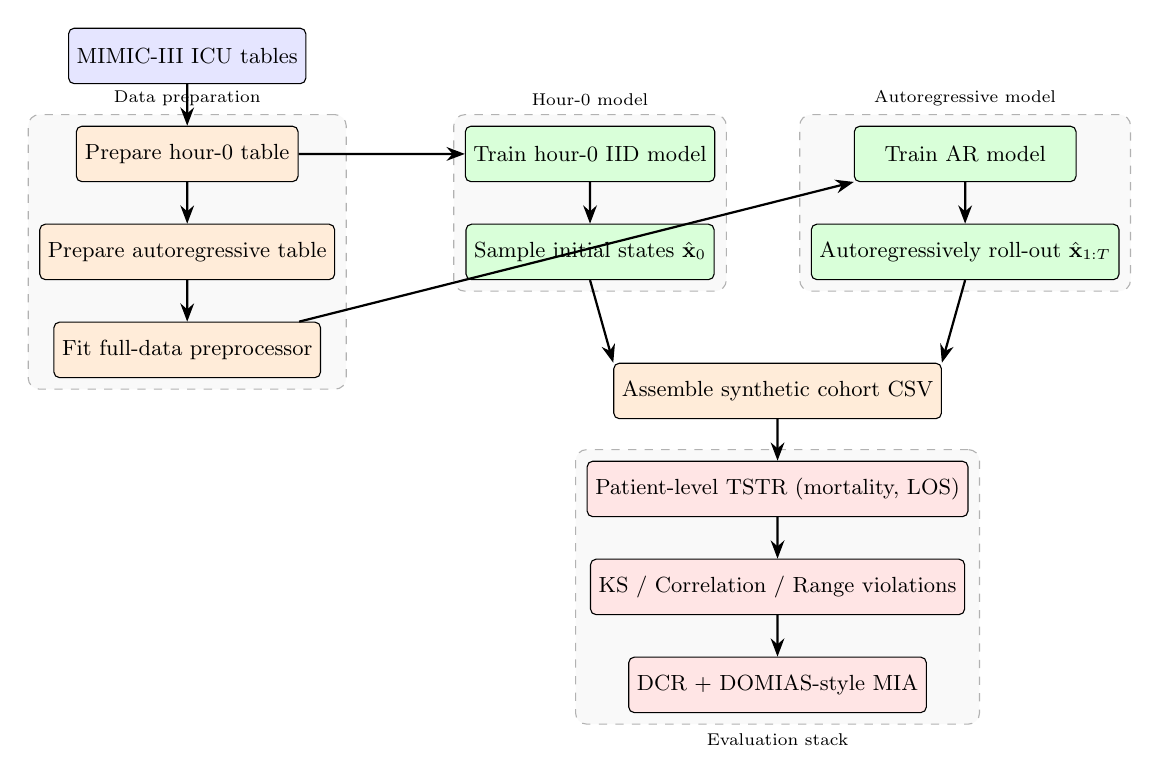
\begin{tikzpicture}[scale=0.88, transform shape,
  node distance = 6mm and 12mm,
  box/.style = {rectangle, draw, rounded corners=2pt,
                minimum width=32mm, minimum height=8mm,
                text centered, font=\small},
  data/.style = {box, fill=blue!10},
  proc/.style = {box, fill=orange!15},
  model/.style= {box, fill=green!15},
  eval/.style = {box, fill=red!10},
  arr/.style  = {-Stealth, thick},
  grp/.style  = {draw=gray!60, dashed, rounded corners=4pt,
                 inner sep=4pt, fill=gray!5}
]

% ,  Data preparation column (left) ,
\node[data]  (mimic)   {MIMIC-III ICU tables};
\node[proc,  below=of mimic]  (p00)    {Prepare hour-0 table};
\node[proc,  below=of p00]    (p01)    {Prepare autoregressive table};
\node[proc,  below=of p01]    (p01b)   {Fit full-data preprocessor};

% ,  Hour-0 branch (middle column) ,
% Anchored at the height of p00 so both training nodes are at the same level
\node[model, right=24mm of p00]  (h0train)  {Train hour-0 IID model};
\node[model, below=of h0train]   (h0gen)    {Sample initial states $\hat{\mathbf{x}}_0$};

% ,  Autoregressive branch (right column, same top height as h0 branch) ,
\node[model, right=20mm of h0train] (artrain)  {Train AR model};
\node[model, below=of artrain]      (argen)    {Autoregressively roll-out $\hat{\mathbf{x}}_{1:T}$};

% ,  Merge: centred between h0gen and argen ,
\node[proc] at ($(h0gen.south)!0.5!(argen.south) + (0,-16mm)$) (merge)
      {Assemble synthetic cohort CSV};

% ,  Evaluation stack (below merge) ,
\node[eval, below=of merge] (tstr)   {Patient-level TSTR (mortality, LOS)};
\node[eval, below=of tstr]  (qual)   {KS / Correlation / Range violations};
\node[eval, below=of qual]  (priv)   {DCR + DOMIAS-style MIA};

% ,  Arrows: data prep ,
\draw[arr] (mimic) -- (p00);
\draw[arr] (p00)   -- (p01);
\draw[arr] (p01)   -- (p01b);

% ,  Arrows: data prep → branches ,
\draw[arr] (p00)   -- (h0train);
\draw[arr] (p01b)  -- (artrain);

% ,  Arrows: within branches ,
\draw[arr] (h0train) -- (h0gen);
\draw[arr] (artrain) -- (argen);

% ,  Arrows: converge to merge ,
\draw[arr] (h0gen.south) -- (merge.north west);
\draw[arr] (argen.south) -- (merge.north east);

% ,  Arrows: evaluation ,
\draw[arr] (merge) -- (tstr);
\draw[arr] (tstr)  -- (qual);
\draw[arr] (qual)  -- (priv);

% ,  Grouping boxes ,
\begin{scope}[on background layer]
  \node[grp, fit=(p00)(p01)(p01b), label=above:{\scriptsize Data preparation}] {};
  \node[grp, fit=(h0train)(h0gen), label=above:{\scriptsize Hour-0 model}] {};
  \node[grp, fit=(artrain)(argen), label=above:{\scriptsize Autoregressive model}] {};
  \node[grp, fit=(tstr)(qual)(priv), label=below:{\scriptsize Evaluation stack}] {};
\end{scope}

\end{tikzpicture}
\caption{End-to-end pipeline. MIMIC-III ICU tables feed two parallel training paths: an IID hour-0 model (generating initial patient states) and an autoregressive transition model (generating subsequent hourly observations). Their outputs are chained into a synthetic cohort CSV, which is passed through the three-axis evaluation stack.}
\label{fig:pipeline-overview}
\end{figure}

\subsection{ForestFlow Architecture}

Figure~\ref{fig:forestflow-arch} shows how ForestFlow is instantiated in this system. The formal flow-matching equations are defined in Chapter~4; here the design point is implementation-facing: one regressor bank per time level, clean conditioning, and Euler rollout for generation.

% , , , , , , , , , , , , , , , , , , , , , , , , ,
% Figure 2: ForestFlow backbone
% , , , , , , , , , , , , , , , , , , , , , , , , ,
\begin{figure}[htbp]
\centering
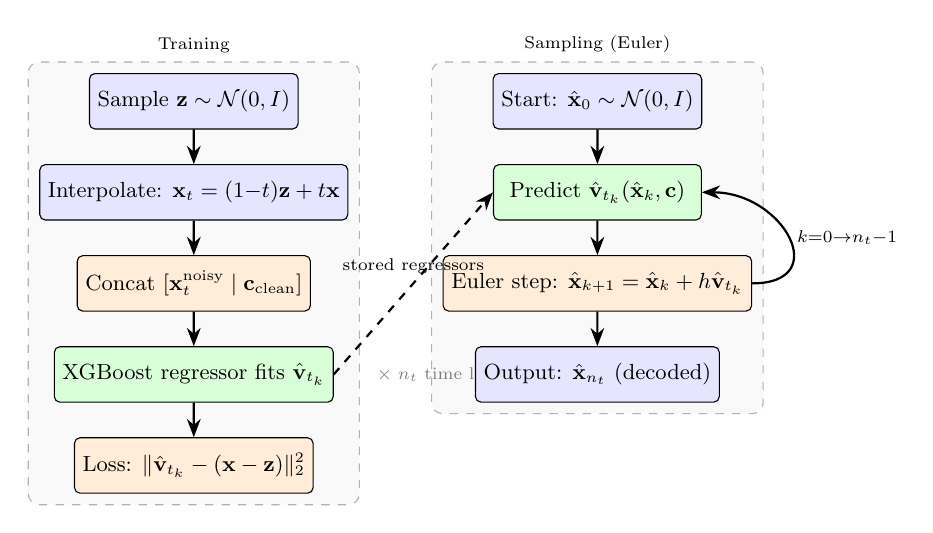
\begin{tikzpicture}[scale=0.88, transform shape,
  node distance = 5mm and 12mm,
  box/.style  = {rectangle, draw, rounded corners=2pt,
                 minimum width=30mm, minimum height=8mm,
                 text centered, font=\small},
  blue/.style = {box, fill=blue!10},
  orange/.style={box, fill=orange!15},
  green/.style ={box, fill=green!15},
  red/.style   ={box, fill=red!10},
  arr/.style   = {-Stealth, thick},
  darr/.style  = {-Stealth, thick, dashed},
  grp/.style   = {draw=gray!60, dashed, rounded corners=4pt,
                  inner sep=4pt, fill=gray!5}
]

% , - Training path (left column) , -
\node[blue]   (noise)  {Sample $\mathbf{z}\sim\mathcal{N}(0,I)$};
\node[blue,   below=of noise]   (interp) {Interpolate: $\mathbf{x}_t=(1{-}t)\mathbf{z}+t\mathbf{x}$};
\node[orange, below=of interp]  (concat) {Concat $[\mathbf{x}_t^{\text{noisy}} \mid \mathbf{c}_{\text{clean}}]$};
\node[green,  below=of concat]  (xgb)    {XGBoost regressor fits $\hat{\mathbf{v}}_{t_k}$};
\node[orange, below=of xgb]     (loss)   {Loss: $\|\hat{\mathbf{v}}_{t_k}-(\mathbf{x}-\mathbf{z})\|_2^2$};

% , - Time loop annotation , -
\node[right=5mm of xgb, font=\scriptsize, text=gray] (timeann)
      {$\times\; n_t$ time levels};

% , - Sampling path (right column) , -
\node[blue,   right=28mm of noise]   (znoise) {Start: $\hat{\mathbf{x}}_0\sim\mathcal{N}(0,I)$};
\node[green,  below=of znoise]       (pred)   {Predict $\hat{\mathbf{v}}_{t_k}(\hat{\mathbf{x}}_k,\mathbf{c})$};
\node[orange, below=of pred]         (euler)  {Euler step: $\hat{\mathbf{x}}_{k+1}=\hat{\mathbf{x}}_k+h\hat{\mathbf{v}}_{t_k}$};
\node[blue,   below=of euler]        (out)    {Output: $\hat{\mathbf{x}}_{n_t}$ (decoded)};

% , - Arrows: training , -
\draw[arr] (noise)  -- (interp);
\draw[arr] (interp) -- (concat);
\draw[arr] (concat) -- (xgb);
\draw[arr] (xgb)    -- (loss);

% , - Arrows: sampling , -
\draw[arr] (znoise) -- (pred);
\draw[arr] (pred)   -- (euler);
\draw[arr] (euler)  to[out=0,in=0,looseness=2]
           node[right,font=\scriptsize]{$k{=}0{\to}n_t{-}1$} (pred);
\draw[arr] (euler)  -- (out);

% , - Training → Sampling arrow , -
\draw[darr] (xgb.east) -- node[above,font=\scriptsize]{stored regressors} (pred.west);

% , - Group boxes , -
\begin{scope}[on background layer]
  \node[grp, fit=(noise)(interp)(concat)(xgb)(loss),
        label=above:{\scriptsize Training}] {};
  \node[grp, fit=(znoise)(pred)(euler)(out),
        label=above:{\scriptsize Sampling (Euler)}] {};
\end{scope}

\end{tikzpicture}
\caption{ForestFlow backbone. \textit{Training}: for each time level $t_k$, the target is interpolated with Gaussian noise and a regressor is fitted to predict the flow direction. \textit{Sampling}: starting from noise, $n_t$ first-order Euler steps integrate the learned vector field back to data space. All target dimensions are treated as continuous flows.}
\label{fig:forestflow-arch}
\end{figure}

\subsection{HS3F Architecture}

Figure~\ref{fig:hs3f-arch} shows the HS3F system design. Chapter~4 defines the formal heterogeneous factorisation; this section focuses on architecture: type-routed heads, feature-wise left-to-right generation, and explicit prefix feedback during sampling.

% , , , , , , , , , , , , , , , , , , , , , , , , ,
% Figure 3: HS3F backbone
% , , , , , , , , , , , , , , , , , , , , , , , , ,
\begin{figure}[htbp]
\centering
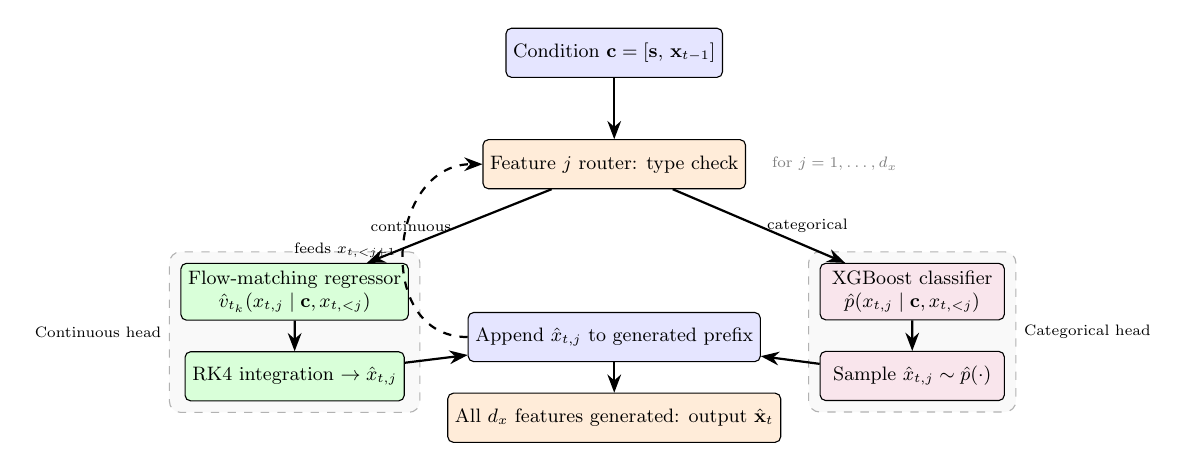
\begin{tikzpicture}[scale=0.78, transform shape,
  node distance = 5mm and 10mm,
  box/.style   = {rectangle, draw, rounded corners=2pt,
                  minimum width=30mm, minimum height=8mm,
                  align=center, font=\small},
  blue/.style  = {box, fill=blue!10},
  orange/.style= {box, fill=orange!15},
  green/.style = {box, fill=green!15},
  purple/.style= {box, fill=purple!10},
  red/.style   = {box, fill=red!10},
  arr/.style   = {-Stealth, thick},
  darr/.style  = {-Stealth, thick, dashed},
  grp/.style   = {draw=gray!60, dashed, rounded corners=4pt,
                  inner sep=4pt, fill=gray!5}
]

% , - Shared input , -
\node[blue]   (cond)  {Condition $\mathbf{c} = [\mathbf{s},\, \mathbf{x}_{t-1}]$};

% , - Feature loop head (router) , -
\node[orange, below=10mm of cond]  (router) {Feature $j$ router: type check};
\node[right=3mm of router, font=\scriptsize, text=gray]
     (loopann) {for $j=1,\ldots,d_x$};

% , - Continuous branch , -
\node[green, below left=12mm and 12mm of router]  (flow)
     {Flow-matching regressor\\$\hat{v}_{t_k}(x_{t,j}\mid\mathbf{c},x_{t,<j})$};
\node[green, below=of flow] (rk4)
     {RK4 integration $\to \hat{x}_{t,j}$};

% , - Categorical branch , -
\node[purple, below right=12mm and 12mm of router] (clf)
     {XGBoost classifier\\$\hat{p}(x_{t,j}\mid\mathbf{c},x_{t,<j})$};
\node[purple, below=of clf] (sample)
     {Sample $\hat{x}_{t,j}\sim\hat{p}(\cdot)$};

% , - Accumulate , -
\node[blue, below=20mm of router]  (accum)
     {Append $\hat{x}_{t,j}$ to generated prefix};
\node[orange, below=of accum] (done)
     {All $d_x$ features generated: output $\hat{\mathbf{x}}_t$};

% , - Arrows , -
\draw[arr] (cond)   -- (router);
\draw[arr] (router) -- node[left, font=\scriptsize]{continuous} (flow);
\draw[arr] (router) -- node[right,font=\scriptsize]{categorical} (clf);
\draw[arr] (flow)   -- (rk4);
\draw[arr] (clf)    -- (sample);
\draw[arr] (rk4)    -- (accum);
\draw[arr] (sample) -- (accum);
\draw[arr] (accum)  -- (done);
% Feedback: generated feature feeds back into condition for next j
\draw[darr] (accum.west) to[out=180,in=180,looseness=1.4]
            node[left,font=\scriptsize]{feeds $x_{t,<j+1}$} (router.west);

% , - Group boxes , -
\begin{scope}[on background layer]
  \node[grp, fit=(flow)(rk4), label=left:{\scriptsize Continuous head}] {};
  \node[grp, fit=(clf)(sample),  label=right:{\scriptsize Categorical head}] {};
\end{scope}

\end{tikzpicture}
\caption{HS3F backbone. Features are generated sequentially in a fixed order. Continuous features are produced by a flow-matching regressor integrated with RK4 by default (explicit Euler is also selectable at sampling time); categorical features are produced by an XGBoost classifier with multinomial sampling. Each generated feature is appended to the conditioning prefix before the next feature is generated, capturing inter-feature dependencies.}
\label{fig:hs3f-arch}
\end{figure}

\subsection{Backbone Selection}

Backbone selection is exposed at training time, with HS3F as the default; operational invocation details are documented in the Implementation chapter.

\subsection{ForestFlow Design Interface}

ForestFlow consumes a target matrix, a clean condition matrix, and feature-type metadata, and emits synthetic targets in transformed coordinates.
The implementation-level rule is simple: all target dimensions are routed through continuous flow regressors to keep interpolation arithmetic well defined.
This keeps the training path uniform but can reduce categorical fidelity; that risk is evaluated in Chapter~7.

\subsection{HS3F Design Interface}

HS3F consumes the same target/condition matrices plus feature typing, and emits synthetic targets in transformed coordinates.
Its implementation rule is to split continuous and categorical dimensions into separate heads and generate features left-to-right with prefix feedback.
Label remapping is retained so classifier class indices stay consistent under subsampling; this prevents index mismatch failures during sampling.

\subsection{Hour-0 + Autoregressive Coupling}

The architecture is intentionally two-stage:
\begin{enumerate}\tightlist
    \item Hour-0 IID model learns initial states.
    \item Autoregressive model learns transitions conditioned on lagged dynamics and static covariates.
\end{enumerate}

This decomposition separates structural initialization from transition dynamics more explicitly than a single model that must infer both jointly.

\paragraph{Sweep-level design.}
Sweep-level design, the hyperparameter protocol, transformed-matrix caching, and canonical result schema, is part of the operational pipeline rather than the generator architecture, and is specified in the Implementation chapter (see~\ref{sec:unified-sweep}).

%==============================================================================
\section{Design Rationale and Trade-offs}
%==============================================================================

\subsection{Why Raw Numeric Pass-Through?}

Tree boosting is split-based and generally robust to monotonic scaling transformations \cite{chen2016xgboost}.
Removing mandatory min-max scaling is intended to simplify preprocessing and reduce opportunities for inverse-transform coupling errors.

\subsection{Why Keep Inverse Transform?}

Even with simplified encoding, inverse transformation remains important for:
\begin{itemize}\tightlist
    \item readable synthetic table export,
    \item downstream evaluator compatibility,
    \item sanity checks in clinical units.
\end{itemize}

\subsection{Why Multi-Backbone Support?}

Forest-Flow \cite{jolicoeur2023forest} remains a well-established baseline and compatibility path.
HS3F \cite{akazan2024hs3f} is the default backbone; its literature positioning is reviewed in Chapter~\ref{ch:background}.

\subsection{Why Preserve Explicit Metadata Artifacts?}

Persisting split metadata and model type in pickled artifacts enables:
\begin{itemize}\tightlist
    \item backward-compatible loading in generation scripts,
    \item reproducible sweep reruns,
    \item traceable migration between architecture revisions.
\end{itemize}

Having justified the system architecture and design trade-offs, the next chapter documents how these design choices were implemented and made reproducible.

\chapter{Implementation}
\label{ch:implementation}

%==============================================================================
\section{Traceability of Objectives to Evidence}
%==============================================================================

Software and systems requirements practice treats bidirectional traceability, from stakeholder needs through design to verification evidence, as a core quality activity \cite{ieee29148Requirements2018}.
Table~\ref{tab:obj-trace} summarises how the objectives of this thesis (hour-0 plus autoregressive ICU synthesis, mixed-type tabular handling, utility/distributional/privacy checks, reproducible logging) map to implementation anchors, evaluation quantities, and the sections below where those links are documented.

\begin{table}[htbp]
\centering
\footnotesize
\setlength{\tabcolsep}{3pt}
\begin{tabularx}{\textwidth}{@{}>{\raggedright\arraybackslash}X >{\raggedright\arraybackslash}X >{\raggedright\arraybackslash}X >{\raggedright\arraybackslash}X@{}}
\toprule
\textbf{Objective / criterion} &
\textbf{Design / implementation} &
\textbf{Metric(s)} &
\textbf{Where evidenced} \\
\midrule
Two-stage synthesis: IID hour~0 then autoregressive rows &
Numbered scripts; \code{run\_sweep} trains both stages per config &
Stage timings; end-to-end sweep rows &
section \textbf{Operational Pipeline}; section \textbf{Unified Sweep Architecture} \\
\midrule
Mixed quantitative / categorical ICU features &
\code{feature\_types} metadata; Forest-Flow vs HS3F paths; label remap in \code{sample()} &
Task inputs after \code{inverse\_transform}; per-column KS on numerics &
section \textbf{Categorical Typing}; section \textbf{Categorical Labels and Flow Integration}; section \textbf{Sampling and Reconstruction} \\
\midrule
Downstream utility of synthetic cohorts &
\code{tstr\_framework} multi-task loop &
Per-task acc., F1, ROC-AUC (macro where noted) &
section \textbf{Multi-Task TSTR}; section \textbf{Task Metrics}; Figures~\ref{fig:sweep_mort_roc}--\ref{fig:sweep_mort_f1} \\
\midrule
Distributional fidelity beyond single-task scores &
Sweep post-process: marginals, correlation gap, clinical bounds &
$\overline{\mathrm{KS}}$, $\|\Delta C\|_F$, range-violation \% &
section \textbf{Distributional Quality Metrics}; section \textbf{Empirical Outcomes from the Hyperparameter Sweep} \\
\midrule
Privacy-preservation risk checks &
\code{src/lexisflow/evaluation/privacy\_metrics.py} (DCR + membership attack) &
DCR median/match rate; baseline/overfit scores; MIA ROC-AUC &
section \textbf{Privacy Risk Metrics}; section \textbf{Key Implementation File Map} \\
\midrule
Reproducibility and auditable experiment history &
Seeds; artifact paths; canonical CSV schema; cache signatures; failure rows preserved &
Logged metrics; \code{degenerate\_flag}; resumable \code{sweep\_results.csv} &
section \textbf{Reproducibility and Reporting Conventions}; section \textbf{Unified Sweep Architecture} \\
\bottomrule
\end{tabularx}
\caption{Objective-to-evidence traceability for this implementation chapter (section titles refer to headings within this chapter).}
\label{tab:obj-trace}
\end{table}

%==============================================================================
\section{Operational Pipeline for Hyperparameter Sweep}
%==============================================================================

The current end-to-end workflow is implemented as numbered scripts with explicit artifacts:
\begin{enumerate}\tightlist
    \item \code{prepare\_hour0.py} and \code{fit\_hour0\_preprocessor.py}
          prepare and encode hour-0 training data.
    \item \code{train\_hour0.py} trains an IID generator.
    \item \code{prepare\_autoregressive.py} creates autoregressive tabular rows and carves patient-disjoint train / test / holdout splits (\code{autoregressive\_data.csv}, \code{real\_test.csv}, \code{real\_holdout.csv}).
    \item \code{fit\_autoregressive\_preprocessor.py} fits the full-data autoregressive preprocessor on the training cohort.
    \item \code{train\_autoregressive.py} trains the autoregressive generator.
    \item \code{generate.py} loads model artifacts and exports synthetic samples.
    \item \code{run\_sweep.py} performs unified hour-0 + autoregressive hyperparameter search.
\end{enumerate}

The architecture is explicitly two-stage and backbone-selectable (\code{forest-flow} or \code{hs3f}, default \code{hs3f}). Quality and TSTR evaluation are integrated directly into \code{run\_sweep.py}; ad-hoc inspection of specific generated outputs is handled by the helpers in \code{synth\_gen.evaluation}. A dedicated matched-cell driver (\code{run\_backbone\_comparison.py}) executes the same data and metric pipeline for HS3F, ForestFlow, and CTGAN at a fixed comparison cell; results are reported in the Evaluation chapter (section~\ref{sec:backbone-comparison}).
This structure was chosen so each sweep row is an auditable end-to-end experiment unit, which is why Chapter~7 can compare utility, fidelity, privacy, and runtime from one consistent log schema.

%==============================================================================
\section{Training Implementation Details}
%==============================================================================

\subsection{Hour-0 IID Training}

\code{train\_hour0.py} loads \code{models/hour0\_preprocessor.pkl}, transforms all hour-0 rows, and fits an IID generator:
\begin{equation}
\hat{p}(\mathbf{z}_0), \quad \mathbf{z}_0=[\mathbf{s},\mathbf{x}_0].
\end{equation}

The script persists model metadata including \code{model\_type}, training hyperparameters, and preprocessor linkage.
This stage exists to model initial-state realism separately from transition dynamics, which explains later findings where rollout quality and hour-0 plausibility diverge.

\subsection{Autoregressive Training}

\code{train\_autoregressive.py} loads \code{models/preprocessor\_full.pkl}, transforms selected rows of \code{autoregressive\_data.csv}, and reconstructs split matrices via persisted indices:
\begin{equation}
X_{\text{target}} = X[:, \text{target\_indices}], \quad
X_{\text{condition}} = X[:, \text{condition\_indices}].
\end{equation}

This removes the previous dependence on naive prefix slicing and is needed in the current implementation when transformed columns are type-grouped.
The design choice prevents target/condition leakage from column-order assumptions, which directly supports the validity of the reported TSTR and fidelity metrics.

\subsection{Categorical Typing Interface}

Both backbones receive \code{feature\_types} from preprocessor metadata:
\begin{itemize}\tightlist
    \item \code{'q'} quantitative,
    \item \code{'c'} categorical.
\end{itemize}

Forest-Flow internally overrides noised target dimensions to quantitative mode (flow arithmetic constraint), while HS3F keeps explicit categorical heads \cite{akazan2024hs3f}.
This was implemented to keep both backbones compatible with one data interface while preserving HS3F's mixed-type path, which is why later backbone differences are interpretable as modelling effects rather than pipeline mismatch.

\subsection{Categorical Labels and Flow Integration (Codebase)}

For HS3F categorical dimensions, training remaps observed categories to contiguous local class indices for XGBoost multiclass fitting; \code{sample()} inverts that map via stored \code{local\_to\_orig} so synthetic rows use the same encoded IDs as the preprocessor artifact.
The training remap yields contiguous class indexing under arbitrary subsampling without sparse multiclass labels at fit time.

For continuous targets under Forest-Flow, sampling follows explicit first-order integration.
Forest-Flow integrates the backward flow with explicit Euler updates (\code{X\_t += h * Y\_hat}) in \code{src/lexisflow/models/forest\_flow.py}.
HS3F continuous dimensions default to \code{solver="rk4"} in \code{src/lexisflow/models/hs3f.py}, with \code{solver="euler"} available as an alternative.

%==============================================================================
\section{Sampling and Reconstruction}
%==============================================================================

\subsection{Model-Space Sampling}

For conditional generation, models sample:
\begin{equation}
\tilde{X}_{\text{target}} \sim p_{\theta}(X_{\text{target}} \mid X_{\text{condition}}).
\end{equation}

In sweep mode, conditioning rows are sampled from the real transformed condition matrix and reused as context for synthetic targets.

\subsection{Rebuilding Full Feature Vectors}

The implementation reconstructs full transformed rows in preprocessor order:
\begin{equation}
X_{\text{full}}[:,\text{target\_indices}] \leftarrow \tilde{X}_{\text{target}}, \quad
X_{\text{full}}[:,\text{condition\_indices}] \leftarrow X_{\text{condition}}.
\end{equation}

Then \code{inverse\_transform()} restores tabular values and category labels.
This reconstruction step is required so all downstream evaluators operate in comparable tabular semantics rather than backbone-specific latent coordinates.

\subsection{Post-Decode Clinical Normalisation}

Known intervention indicators (e.g., \code{vent}, \code{vaso}) are explicitly clipped/rounded to $\{0,1\}$ before evaluation/export.
This step is intended to restore discrete $\{0,1\}$ semantics for binary treatment flags after decode.

%==============================================================================
\section{Evaluation Stack}
%==============================================================================

\subsection{Cohort-Level Data Splits}
\label{sec:cohort-splits}

All utility, fidelity, and privacy metrics are computed against real-data cohorts that are patient-disjoint from the generator's training cohort.
At preprocessing time (\code{scripts/prepare\_autoregressive.py}), the autoregressive table is partitioned at the \code{subject\_id} level into three CSVs with an 80\,/\,10\,/\,10 split drawn from a fixed RNG seed so the partition is reproducible across runs:
\begin{itemize}\tightlist
    \item \code{data/processed/autoregressive\_data.csv} -- the training cohort (80\,\% of patients), the only file the generator ever sees.
    \item \code{data/processed/real\_test.csv} -- a TSTR / fidelity reference cohort (10\,\% of patients).
    \item \code{data/processed/real\_holdout.csv} -- a privacy-evaluation holdout cohort (10\,\% of patients).
\end{itemize}

Because the split is performed on \code{subject\_id}, no patient's timesteps ever span the training cohort and an evaluation cohort.
Consequently:
\begin{itemize}\tightlist
    \item Multi-task TSTR (section \textbf{Multi-Task TSTR}) trains classifiers on synthetic data and tests them on sequences drawn from \code{real\_test.csv}; the real-trained baseline classifier is also fit and evaluated entirely within this disjoint cohort via an internal stratified split (\code{test\_size=0.3}).
    \item The distributional fidelity metrics (KS, correlation Frobenius norm, range-violation rate) are computed against a sample of \code{real\_test.csv} rather than the training matrix, so they measure distributional recovery of \emph{unseen} rows rather than reproduction of the training set.
    \item The DCR overfitting-protection and DOMIAS-style membership-inference attack use \code{real\_holdout.csv} directly as the holdout reference, giving the overfitting-vs-generalisation comparison a meaningful signal even when the generator is expressive enough to memorise.
\end{itemize}

The split is materialised once per preprocessing run and referenced explicitly by \code{AutoregressiveInputs.real\_test\_path} and \code{AutoregressiveInputs.real\_holdout\_df} in \code{src/lexisflow/sweep/data\_prep.py}, ensuring the sweep driver, the matched backbone-comparison driver, and any future evaluation scripts consume byte-identical reference cohorts.

\subsection{Multi-Task TSTR}

The active sweep uses a unified patient-level TSTR framework with two tasks:
\begin{enumerate}\tightlist
    \item Mortality classification (binary, patient-level),
    \item ICU LOS category classification (multi-class, patient-level).
\end{enumerate}

Each task uses a \code{\_PaddedSequenceClassifier}: patient trajectories are grouped by \code{subject\_id}, sorted by \code{hours\_in}, padded to a common length with a binary mask, flattened, and fed to a logistic-regression baseline. This patient-level design eliminates within-patient data leakage and captures the temporal structure the autoregressive generator is designed to preserve. The design evolution from the original row-level three-task framework and the rationale for removing vasopressor-use prediction are documented in the Evaluation chapter. The TSTR paradigm follows established synthetic health-data evaluation practice \cite{esteban2018rcgan}.

\subsection{Task Metrics}

For binary tasks, reported metrics include accuracy, F1, and ROC-AUC.
For LOS (multi-class), macro-F1 and one-vs-rest macro ROC-AUC are included.

\subsection{Distributional Quality Metrics}

In addition to task utility, sweep evaluation computes:
\begin{enumerate}\tightlist
    \item Average KS statistic across valid numeric columns,
    \item Correlation matrix Frobenius norm,
    \item Clinical range violation percentage.
\end{enumerate}

Let $\mathcal{J}$ be valid numeric columns:
\begin{equation}
\text{KS}_{\text{avg}} = \frac{1}{|\mathcal{J}|}\sum_{j\in\mathcal{J}}\sup_x |F_j^{\text{real}}(x)-F_j^{\text{synth}}(x)|.
\end{equation}
\begin{equation}
\text{CorrDiff} = \|C^{\text{real}} - C^{\text{synth}}\|_F.
\end{equation}

Columns with insufficient finite samples or zero variance are excluded before these computations to avoid undefined correlations.

\subsection{Privacy Risk Metrics}

To complement utility/fidelity metrics, the current implementation adds four privacy checks used in recent tabular-synthetic evaluation practice \cite{lautrup2024syntheval,breugel2023domias}:
\begin{enumerate}\tightlist
    \item Distance to Closest Record (DCR) summary ($\mathrm{median}$, tails, exact-match rate),
    \item DCR baseline-protection score (synthetic-vs-random closeness to real data),
    \item DCR overfitting-protection score (synthetic closeness to train vs holdout),
    \item DOMIAS-inspired membership inference attack (MIA) ROC-AUC and attacker advantage.
\end{enumerate}

For synthetic samples $\tilde{x}_i$ and real training set $\mathcal{D}_{\text{train}}$, DCR is:
\begin{equation}
\mathrm{DCR}(\tilde{x}_i,\mathcal{D}_{\text{train}})=\min_{x\in\mathcal{D}_{\text{train}}}\|\phi(\tilde{x}_i)-\phi(x)\|_2,
\end{equation}
with mixed-type embedding $\phi(\cdot)$ (min-max normalised numerics + one-hot categoricals).
Baseline protection follows the SDMetrics ratio form \cite{sdmetricsPrivacyDocs}:
\begin{equation}
\mathrm{Score}_{\text{baseline}}=\min\left(1,\frac{\mathrm{median}\,\mathrm{DCR}_{\text{synth}\rightarrow\text{train}}}{\mathrm{median}\,\mathrm{DCR}_{\text{random}\rightarrow\text{train}}}\right).
\end{equation}

Overfitting protection compares train-vs-holdout nearest-neighbour proximity for synthetic rows, where the holdout is the patient-disjoint \code{real\_holdout.csv} cohort defined in section~\ref{sec:cohort-splits}:
\begin{equation}
\mathrm{Score}_{\text{overfit}}=\min\left(1,\,2\left(1-\Pr\left[\mathrm{DCR}_{\text{synth}\rightarrow\text{train}} < \mathrm{DCR}_{\text{synth}\rightarrow\text{holdout}}\right]\right)\right).
\end{equation}

Membership risk is quantified with a DOMIAS-style local overfitting score \cite{breugel2023domias}:
\begin{equation}
s(x)=\log\frac{d_{\text{ref}}(x)+\epsilon}{d_{\text{synth}}(x)+\epsilon},
\end{equation}
where $d_{\text{synth}}$ is nearest-neighbour distance to synthetic data and $d_{\text{ref}}$ is distance to the patient-disjoint holdout cohort, so a non-zero attacker advantage can only reflect closeness to training patients rather than to the evaluation cohort itself.
Attack performance is reported via ROC-AUC (and attacker advantage) in the membership-inference paradigm \cite{shokri2017membership}.

\paragraph{Interpretation guardrail.}
DCR-style proximity metrics are useful diagnostics but should not be treated as sufficient legal/anonymity evidence on their own; recent work shows distance-only proxies can miss true membership leakage, so MIA results remain primary for privacy claims \cite{yao2025dcrdelusion}.

\subsection{Empirical Outcomes from the Hyperparameter Sweep}

The canonical log \code{results/sweep\_results.csv} stores one normalised row per completed sweep cell over the configured $(n_t, n_{\text{noise}})$ grid. The schema includes metric columns, stage timings, error fields, and optional uncertainty fields (\code{*\_std}, \code{*\_ci95}, \code{trajectory\_seed\_count}) for multi-seed runs.

This chapter documents how those values are produced and persisted. The interpretation of utility, fidelity, privacy, and efficiency outcomes is intentionally centralised in Chapter~7.

\paragraph{Trajectory-Level Coherence Metrics}
\label{sec:trajectory-coherence}

The trajectory-level metrics defined in Chapter~7 (autocorrelation distance, stay-length KS, transition smoothness ratio, temporal cross-feature drift) are implemented in \code{src/lexisflow/evaluation/trajectory\_metrics.py} and integrated into \code{run\_sweep.py}, with dedicated unit coverage in \code{src/lexisflow/evaluation/tests/test\_trajectory\_metrics.py}. Implementation correctness is established by tests that verify:
\begin{itemize}\tightlist
    \item zero values when real and synthetic trajectories are identical (sanity bound);
    \item monotonic degradation as synthetic trajectories are perturbed with progressively larger noise;
    \item stable behaviour when trajectory lengths fall below the minimum window (short trajectories are excluded rather than causing NaNs).
\end{itemize}
Numerical results and interpretation are reported in Chapter~7.

%==============================================================================
\section{Unified Sweep Architecture}
\label{sec:unified-sweep}
%==============================================================================

\subsection{Per-Configuration Lifecycle}

For each $(n_t, n_{\text{noise}})$ pair, \code{run\_sweep.py} executes:
\begin{enumerate}\tightlist
    \item Train hour-0 IID model,
    \item Train autoregressive model,
    \item Generate synthetic samples,
    \item Run multi-task TSTR + quality metrics,
    \item Append one normalised CSV row.
\end{enumerate}

Each finished configuration is normalised to the canonical header list \code{SWEEP\_RESULT\_COLUMNS} before append, so partial reruns do not corrupt \code{results/sweep\_results.csv}.
The row payload includes utility metrics, quality metrics, timing fields for both model stages, and \code{degenerate\_flag}.

\subsection{Always-On Transformed Cache}

Autoregressive transformed arrays are cached by default under \code{models/sweep\_cache/transformed\_autoregressive/} and reloaded when a signature check passes.

The signature dict in \code{metadata.pkl} is produced by \code{\_build\_cache\_signature} in \code{run\_sweep.py}: CSV path, size, and nanosecond mtime; \code{n\_cols} and \code{n\_target}; SHA-256 hashes of the ordered column-name list, \code{target\_indices}, and \code{condition\_indices}.
\code{\_load\_transformed\_cache} requires exact equality of all signature fields before reusing cached \code{.npy} arrays.

A hit skips redundant \code{transform} work; a miss rebuilds matrices and overwrites the cache, preventing reuse after the input file, schema, or index split changes.

\subsection{Resumability and Failure Logging}

Runs are keyed by \code{(nt, n\_noise)} from \code{results/sweep\_results.csv}; any existing row for a key is skipped on rerun, including rows previously written after failures.
Failures do not abort the full sweep; they are written as explicit NaN/error rows, preserving an audit trail.

\subsection{Degeneracy Guardrail}

A run is flagged as degenerate when both patient-level synthetic-side thresholds are simultaneously met:
\code{mortality\_synth\_roc\_auc <= 0.55} and \code{los\_synth\_macro\_f1 <= 0.15}, with finite-value checks before thresholding.
Vasopressor metrics are no longer part of the degeneracy check following the TSTR framework revision described in the Evaluation chapter.
Importantly, runs are \emph{not} dropped; metrics are preserved and annotated with \code{degenerate\_flag=1}.

%==============================================================================
\section{Reproducibility and Reporting Conventions}
%==============================================================================

The current report and code follow reproducibility-oriented implementation practices:
\begin{itemize}\tightlist
    \item deterministic seeds for NumPy/model constructors,
    \item explicit artifact paths and metadata-rich pickles,
    \item canonical CSV schema enforcement before append,
    \item transparent warnings instead of silent failures,
    \item progress instrumentation for long-running stages.
\end{itemize}

These choices are consistent with reproducible computational research practice and are intended to support debugging and thesis traceability.

%==============================================================================
\section{Relationship to External Methods and Projects}
%==============================================================================

Our implementation is grounded in:
\begin{itemize}\tightlist
    \item flow matching for CNF-style training \cite{lipman2023flow},
    \item tree-based flow matching for tabular generation \cite{jolicoeur2023forest},
    \item heterogeneous sequential mixed-type generation \cite{akazan2024hs3f},
    \item XGBoost as the core function approximator \cite{chen2016xgboost}.
\end{itemize}

Common synthetic tabular/time-series baselines include CTGAN \cite{xu2019ctgan}, TimeGAN \cite{yoon2019timegan}, TabDDPM \cite{kotelnikov2023tabddpm}, TabSyn \cite{zhang2024tabsyn}, and SDV ecosystem tooling \cite{sdvproject}. In this project, CTGAN is integrated through \code{src/lexisflow/models/ctgan\_adapter.py} as a pragmatic lower-bound/reference baseline inside the same data and metric pipeline. Transformer-based generators such as GReaT \cite{borisov2023great} and REaLTabFormer \cite{solatorio2023realtabformer} remain future comparison points.

%==============================================================================
\section{Key Implementation Modules}
%==============================================================================

The implementation centres on a small set of modules, each tied to a reported outcome:
\begin{itemize}\tightlist
    \item \code{src/lexisflow/data/transformers.py}: preprocessing/inverse decoding that governs whether generated rows can be evaluated in clinically meaningful units.
    \item \code{src/lexisflow/models/\{forest\_flow,hs3f\}.py}: backbone-specific training/sampling logic that drives fidelity and utility differences.
    \item \code{src/lexisflow/evaluation/\{tstr\_framework,privacy\_metrics,trajectory\_metrics\}.py}: metric implementations that produce the evidence interpreted in Chapter~7.
    \item \code{scripts/\{fit\_autoregressive\_preprocessor,train\_hour0,train\_autoregressive,run\_sweep\}.py}: orchestration layer that makes runs reproducible and sweep results comparable.
\end{itemize}

\chapter{Results/Evaluation}

%==============================================================================
\section{Software Testing}
%==============================================================================

The evaluation subsystem is verified with deterministic unit tests before computationally expensive sweeps are executed. The tests, implemented with \code{pytest} in \code{src/synth\_gen/evaluation/tests/}, target metric correctness, edge-case handling, and report-schema stability \cite{pytestProject}.

\subsection{Quality-Metric Tests}

The following functions are covered:
\begin{itemize}\tightlist
    \item \code{compute\_ks\_statistics},
    \item \code{compute\_correlation\_frobenius},
    \item \code{compute\_clinical\_range\_violations}.
\end{itemize}
These tests check expected behavior under controlled fixtures:
\begin{itemize}\tightlist
    \item identical real/synthetic distributions produce near-zero KS and near-zero correlation-matrix difference;
    \item shifted distributions produce larger KS values;
    \item non-overlapping or insufficient numeric columns return \code{NaN} for correlation metrics rather than failing;
    \item clinical-range checks return exact violation percentages for synthetic fixtures with known out-of-range values.
\end{itemize}

This structure provides an implementation-level regression guard: if code changes alter known outcomes on fixed fixtures, failures are surfaced immediately.

\subsection{Privacy-Metric Tests}

Privacy tests target the principal leakage scenarios represented in \code{privacy\_metrics.py}:
\begin{itemize}\tightlist
    \item duplicate synthetic rows sampled from training data should yield near-zero DCR median and high exact-match rate;
    \item overfitting protection should decrease when synthetic rows are closer to training than holdout data;
    \item DOMIAS-like membership attack scores are expected to exceed chance-level behavior in memorization-heavy fixtures;
    \item integrated reports must always expose all expected sections (\code{dcr\_stats}, baseline/overfitting protection, membership inference).
\end{itemize}

These tests do not constitute a formal privacy proof; they verify that implemented diagnostics react directionally as expected under stress conditions.

\subsection{What Is and Is Not Covered}

The current suite focuses on unit-level correctness and defensive behavior (missing columns, \code{NaN}s, low-sample regimes). End-to-end statistical validity at MIMIC scale is assessed through the sweep protocol and subsequent analysis, rather than per-commit integration tests. This separation is intentional because full-grid experiments are computationally costly.

%==============================================================================
\section{Evaluation Methodology and Metric Rationale}
%==============================================================================

This section specifies the evaluation protocol used in this project. It focuses on methodological design and metric rationale, not numerical outcomes.

\subsection{Sweep-Oriented Evaluation Protocol}

Evaluation is operationalized as a reproducible sweep loop (\code{scripts/run\_sweep.py}) over $(n_t, n_{\text{noise}})$:
\begin{enumerate}\tightlist
    \item train hour-0 IID model and autoregressive model with the same hyperparameters;
    \item generate synthetic rows conditioned on sampled real contexts;
    \item evaluate utility (multi-task TSTR), statistical quality, and privacy;
    \item append one canonical row to \code{results/sweep\_results.csv}.
\end{enumerate}

The sweep is resumable by design (existing rows are skipped), logs failed runs with explicit error fields, and maintains schema compatibility through migration checks. To reduce recomputation, transformed matrices are cached with signatures over source-table metadata and split-index hashes.

\subsection{Baseline Scope and Interpretation}

The evaluation includes a CTGAN/CRGAN-style baseline as a \emph{reference lower bound}, not as a fully matched autoregressive competitor. In the current implementation, CTGAN is trained on the transformed joint table but sampled without per-row autoregressive conditioning. This means it does not consume the full row-specific context vector at generation time in the same way as the ForestFlow and HS3F transition models.

Making CTGAN fully autoregressive in this pipeline would require an architecture-level redesign (for example, a new sequential wrapper with explicit step-wise conditioning logic, state propagation, and compatibility checks across mixed continuous/categorical features), rather than a small hyperparameter or script-level modification. Delivering that redesign with adequate validation would expand the implementation and experiment surface beyond the scope of this thesis.

Accordingly, CTGAN/CRGAN results are interpreted conservatively: they provide a practical baseline reference and lower-bound comparator for utility/quality/privacy trends, but they are not used to make strong claims about parity with fully conditional autoregressive generators.

\subsection{Utility Evaluation via Multi-Task TSTR}

Primary utility assessment follows the Train-on-Synthetic, Test-on-Real (TSTR) paradigm, a widely used protocol in synthetic healthcare-data evaluation \cite{esteban2018rcgan,yan2022benchmarking}. The core idea is to train a downstream clinical predictor on synthetic data only and evaluate it on real held-out patients; the resulting performance gap relative to a real-trained baseline quantifies how much predictive signal the synthetic generator preserves.

\paragraph{Initial design: row-level TSTR.}

The evaluation framework was initially implemented as a row-level TSTR protocol. Each synthetic row (one patient-hour) was treated as an independent training sample; the downstream classifier was a logistic-regression model fitted on individual rows; and the test set was a held-out split of real rows. Three clinical tasks were targeted: mortality prediction, vasopressor-use prediction, and ICU length-of-stay (LOS) category prediction.

While straightforward to implement, this design was found to suffer from four structural pitfalls:

\begin{enumerate}
    \item \textbf{Patient-level data leakage.} Row-level train/test splitting does not respect patient boundaries. Multiple hourly observations from the same patient can appear in both training and evaluation sets. The downstream classifier can then exploit within-patient autocorrelations rather than the quality of the synthetic distribution, inflating TSTR scores independently of generator performance.

    \item \textbf{Temporal structure blindness.} The autoregressive generator is explicitly designed to capture hour-to-hour dynamics within a patient trajectory. Row-level evaluation treats each hourly observation as independent and identically distributed, making it structurally blind to the temporal coherence properties that the generator is meant to preserve. A generator that reproduces correct marginals but entirely wrong temporal dynamics scores the same as a well-calibrated one under this protocol.

    \item \textbf{Vasopressor task degeneration under row-level imbalance.} Vasopressor use is a sparse event: in the MIMIC-III ICU cohort, vasopressors are administered in a minority of patient-hours. At row level, a classifier can achieve high accuracy by predicting the negative class on nearly every row. This pathological majority-class collapse renders the vasopressor task uninformative as a utility signal, and is consistent with the F1 collapse behaviour observed in the sweep results (see Implementation chapter, §\textbf{Empirical Outcomes}).

    \item \textbf{Granularity mismatch with clinical deployment.} Synthetic EHR data is generated for patient-level clinical use---mortality forecasting, LOS prediction, discharge planning. Evaluating at row granularity measures a proxy for this that is misaligned with the actual downstream application context.
\end{enumerate}

\paragraph{Revised design: patient-level sequence TSTR.}

In response to these pitfalls, the TSTR framework was revised to operate at \emph{patient trajectory} level. Let $\mathcal{S}_i = \{\mathbf{x}_{i,0}, \ldots, \mathbf{x}_{i,T_i}\}$ denote the ordered sequence of hourly feature vectors for patient $i$, and let $y_i$ denote the patient-level label. The synthetic-trained sequence classifier $g_{\phi}$ is evaluated as:

\begin{equation}
\phi_{\text{synth}} = \arg\min_{\phi}\mathcal{L}(g_{\phi}(\mathcal{S}_{\text{synth}}), y_{\text{synth}}), \quad
\text{evaluate } g_{\phi_{\text{synth}}} \text{ on } (\mathcal{S}_{\text{real,test}}, y_{\text{real,test}}).
\end{equation}

Patient-level splitting is performed by \code{subject\_id} at two levels. First, the raw MIMIC-III cohort is partitioned once at preprocessing time (\code{scripts/01\_preprocess\_data.py}) into a training cohort (\code{autoregressive\_data.csv}, 80\,\% of patients), a TSTR / fidelity reference cohort (\code{real\_test.csv}, 10\,\% of patients), and a privacy-evaluation holdout cohort (\code{real\_holdout.csv}, 10\,\% of patients); the generator is only ever exposed to the first file, so the real cohorts used for evaluation share no patients with the cohort the generator learned from. Second, within \code{real\_test.csv}, the real patient cohort is split 70\,\% / 30\,\% for the real-trained baseline classifier (implemented as \code{test\_size=0.3} in \code{tstr\_framework.py}), with stratification on the task label where class support permits. All timesteps from one patient remain in the same split at both levels, eliminating within-patient leakage. Sequences are sorted by \code{hours\_in}, padded to a common length with a binary mask, flattened, and fed to a logistic-regression model (implemented as \code{\_PaddedSequenceClassifier} in \code{tstr\_framework.py}). This preserves temporal order and full-stay context per patient without requiring a recurrent or attention-based architecture; the mask encodes which timesteps are genuine observations versus padding.

The vasopressor-use task was removed from the revised framework. At patient level, a binary ``ever received vasopressors'' label is more naturally defined, but vasopressor administration is a well-established marker of haemodynamic instability and septic shock severity that correlates strongly with both in-hospital mortality and prolonged ICU stay \cite{yan2022benchmarking}. As a consequence, a classifier trained to predict vasopressor use tends to recapitulate the same predictive signal as mortality and LOS classifiers, reducing its value as an independent utility dimension. The final framework evaluates two tasks implemented in \code{tstr\_framework.py}:

\begin{itemize}\tightlist
    \item mortality prediction (binary, patient-level),
    \item ICU length-of-stay category prediction (multi-class, patient-level).
\end{itemize}

Task models use class-balanced logistic-regression baselines from scikit-learn \cite{pedregosa2011scikit} with \code{class\_weight="balanced"} to partially compensate for residual class imbalance. Reported metrics include accuracy, F1 (and macro F1 for multi-class), and ROC-AUC (binary or one-vs-rest macro) \cite{fawcett2006roc}. A real-trained baseline (train-real/test-real) is computed in parallel for comparison.

\subsection{Statistical Quality Metrics}

Complementary to TSTR, the project computes feature-space quality metrics in \code{quality\_metrics.py}:
\begin{enumerate}\tightlist
    \item \textbf{Average KS statistic} across common numeric features, via two-sample KS:
    \begin{equation}
    \overline{KS} = \frac{1}{|\mathcal{J}|}\sum_{j\in\mathcal{J}}\sup_x\left|F^{\text{real}}_j(x)-F^{\text{synth}}_j(x)\right|.
    \end{equation}
    \item \textbf{Correlation Frobenius norm}:
    \begin{equation}
    \Delta_{\text{corr}} = \left\|C_{\text{synth}} - C_{\text{real}}\right\|_{F}.
    \end{equation}
    \item \textbf{Clinical range violation percentage} over predefined physiologic bounds.
\end{enumerate}

This metric family aligns with synthetic-EHR benchmarking practice that combines distributional fidelity, relationship preservation, and plausibility checks \cite{yan2022benchmarking,kaabachi2025scoping}. The KS implementation relies on SciPy statistical tooling \cite{virtanen2020scipy}.

\subsection{Privacy Evaluation Metrics}

Privacy assessment in \code{privacy\_metrics.py} combines proximity diagnostics with attack-oriented indicators:
\begin{itemize}\tightlist
    \item DCR summary statistics (\code{median}, low-tail quantiles, exact-match rate),
    \item DCR baseline protection score (synthetic versus random baseline),
    \item DCR overfitting protection score (synthetic closeness to train versus holdout),
    \item DOMIAS-inspired membership inference metrics (ROC-AUC, average precision, attacker advantage).
\end{itemize}

The overfitting-protection and membership-inference metrics require a real reference cohort that the generator has never observed; both consume \code{real\_holdout.csv}, the 10\,\% patient-disjoint holdout carved at preprocessing time, passed into \code{compute\_privacy\_metrics(..., holdout\_df=...)} by the sweep driver. This disjointness is what makes the train-vs-holdout comparison in Score$_{\text{overfit}}$ and the attacker reference distance $d_{\text{ref}}$ in DOMIAS informative: a memorising generator cannot hide by being equally close to training and evaluation patients, because the two cohorts share no subjects.

The DCR-based protection scores follow SDMetrics-style formulations \cite{sdmetricsPrivacyDocs}. Membership inference follows the attack perspective introduced in classical MIA literature and modern synthetic-data attacks \cite{shokri2017membership,breugel2023domias}. Average precision is reported alongside ROC-AUC for ranking quality under class-imbalance sensitivity \cite{davisGoadrich2006}. Recent work also motivates caution: distance-only metrics should not be interpreted as standalone privacy guarantees \cite{yao2025dcrdelusion}.

\subsection{Trajectory-Level Quality Metrics}

The per-row metrics above assess marginal fidelity but cannot detect temporal incoherence within patient trajectories. A generator that produces correct marginal distributions may still fail to capture hour-to-hour dynamics---for example, yielding heart-rate sequences that jump erratically rather than evolving smoothly. To address this gap, the evaluation pipeline includes four trajectory-level metrics implemented in \code{trajectory\_metrics.py}:

\begin{enumerate}\tightlist
    \item \textbf{Autocorrelation distance} (\code{autocorr\_distance}): For each vital sign, the lag-1 autocorrelation is computed per trajectory and summarised by median. The metric reports the mean absolute difference in per-feature median autocorrelation between real and synthetic trajectories. A value of~$0$ indicates that synthetic trajectories preserve real temporal dependency; values above~$\sim 0.3$ indicate substantial structure loss.

    \item \textbf{Stay-length KS statistic} (\code{stay\_length\_ks}): A two-sample Kolmogorov--Smirnov test on the distribution of trajectory lengths (rows per \code{subject\_id}). Because the current generator produces fixed 48-hour trajectories while real ICU stays vary in length, this metric quantifies a known structural limitation of the fixed-window autoregressive scheme.

    \item \textbf{Transition smoothness ratio} (\code{transition\_mse\_ratio}): The ratio of mean hourly absolute change in each vital sign, synthetic versus real. A ratio of~$1.0$ means transitions are equally smooth; values above~$1$ indicate rougher (jumpier) synthetic trajectories; values below~$1$ indicate over-smoothed trajectories.

    \item \textbf{Temporal cross-feature correlation drift} (\code{temporal\_corr\_drift}): For clinically meaningful feature pairs (heart rate vs.\ MAP, systolic vs.\ diastolic BP, SpO\textsubscript{2} vs.\ respiratory rate), the within-trajectory Pearson correlation is computed per patient, and the metric reports the mean absolute difference in median correlation between real and synthetic data. This captures whether the generator preserves physiological relationships \emph{within} individual trajectories, not just in aggregate.
\end{enumerate}

These metrics are computed before per-row quality metrics in the sweep loop, using the raw DataFrames that retain \code{subject\_id} and \code{hours\_in} for grouping. Trajectories shorter than four timesteps are excluded to ensure stable autocorrelation estimates. Seed-level uncertainty (mean, standard deviation, CI95) is defined in the \code{SWEEP\_RESULT\_COLUMNS} schema and is populated whenever the trajectory-sampling seed list \code{TSTR\_TRAJECTORY\_SAMPLING\_SEEDS} in \code{run\_sweep.py} has length greater than one. Each entry in that list drives both the trajectory-sampling RNG and the evaluator \code{random\_state} (real/synthetic train-test split, real-baseline classifier, and privacy-attack subsampling), so the reported \code{\_std} and \code{\_ci95} columns reflect compounded trajectory and evaluator variance rather than trajectory variance alone. In the results reported here, the three-seed protocol is exercised at the matched backbone-comparison cell; the main-grid canonical CSV is currently single-seed, and its point estimates should be treated as trend-level rather than statistically bounded.

\subsection{Model-Screening Guardrail}

To reduce accidental over-interpretation of clearly weak runs, the sweep records a \code{degenerate\_flag} when the two patient-level synthetic-side utility metrics are simultaneously near-random: mortality ROC-AUC $\leq 0.55$ and LOS macro-F1 $\leq 0.15$. This is an experiment-management heuristic and is not used as a formal inferential criterion; flagged rows are retained in the sweep CSV rather than dropped, preserving an audit trail of degenerate configurations.

\subsection{Reporting Scope}

This chapter defines the \emph{evaluation protocol}. Numerical outcomes across the full hyperparameter sweep grid are presented in the Implementation chapter (\S~\textbf{Empirical Outcomes from the Hyperparameter Sweep}). The remainder of this chapter provides a figure-by-figure interpretation of the sweep plots in \code{results/sweep\_plots/}, grounded in the aggregated values in \code{results/sweep\_results.csv}, followed by an extrapolation to the production configuration $(n_t, n_{\text{noise}})=(50, 100)$.

%==============================================================================
\section{Empirical Analysis of the Hyperparameter Sweep}
%==============================================================================

\subsection{Scope and Caveats}

The analysis below covers the Fibonacci-scale grid $n_t, n_{\text{noise}} \in \{1, 2, 3, 5, 8, 13, 21, 34\}$. At the time of writing, 52 of 64 cells are complete; the $n_t{=}21$ row is populated up to $n_{\text{noise}}{=}8$, and the $n_t{=}34$ row is not yet populated. Every figure is therefore analysed within that populated envelope, and statements about the top-right quadrant of each heatmap are marked accordingly. Each reported cell aggregates three trajectory-sampling seeds; reported standard deviations therefore reflect only within-cell trajectory and evaluator variance, not across-cell stochastic training variance (the generator itself is trained once per cell).

A structural caveat applies throughout: the real-model TSTR baselines (mortality ROC-AUC $\approx 0.82$, LOS macro-F1 $\approx 0.77$) are computed on a patient-disjoint subset of \code{real\_test.csv} using the same logistic-regression sequence classifier as the synthetic-trained arm. They are therefore a tight upper bound for what a linear classifier can extract from this cohort, not an absolute ceiling---a non-linear classifier would raise the baseline further, which would in turn widen every gap reported below.

\subsection{Mortality TSTR: ROC-AUC, Accuracy, Balanced Accuracy, and F1}

\begin{figure}[h]\centering

\includegraphics[width=\textwidth]{sweep_heatmap.png}
\caption{Mortality TSTR ROC-AUC across the sweep grid (left) and the gap against the real-trained baseline (right). White cells are not yet populated.}
\label{fig:sweep_mort_roc}
\end{figure}

ROC-AUC is the most scientifically informative mortality metric in this regime because (i) the cohort is class-imbalanced and (ii) the synthetic-trained classifier frequently collapses to near-constant predictions, which inflates or deflates threshold-dependent metrics. Figure~\ref{fig:sweep_mort_roc} shows a clean monotone signal in $n_t$: ROC-AUC rises from $0.47$--$0.52$ at $n_t{=}1$ to $0.63$--$0.66$ at $n_t{\geq}8$, then plateaus. Across the $n_{\text{noise}}$ axis the same row is essentially flat (marginal means differ by $< 0.02$ between $n_{\text{noise}}{=}1$ and $n_{\text{noise}}{=}34$). The gap-to-real panel mirrors this: $-0.35$ at the sparsest cell, narrowing to $-0.17$ at the best cell, but never closing.

The interpretation is that $n_t$ controls the fidelity of the flow-matching integration path: with too few integration steps the target distribution is under-fit and predictors trained on the resulting samples carry almost no class signal. $n_{\text{noise}}$ controls the number of noise anchors per training row, which in principle should regularise the score-matching objective, but in this pipeline the downstream TSTR task is dominated by bias, not variance: adding noise anchors cannot rescue a mis-integrated velocity field. This is an architectural rather than a hyperparameter finding, and it implies that spending compute on larger $n_{\text{noise}}$ is poor value unless $n_t$ is already in the saturated region.

\begin{figure}[h]\centering

\includegraphics[width=\textwidth]{sweep_f1_heatmap.png}
\caption{Mortality TSTR F1 (left) and gap against the real-trained baseline (right).}
\label{fig:sweep_mort_f1}
\end{figure}

F1 on the mortality task (Figure~\ref{fig:sweep_mort_f1}) tells a more pessimistic story: values sit in $0.1$--$0.22$ against a real-model baseline of $\approx 0.47$, and the gap barely closes with $n_t$. This is consistent with a synthetic generator that preserves \emph{rank ordering} (which ROC-AUC measures) but systematically mis-calibrates the decision threshold. In other words, the synthetic mortality signal is directionally correct but the positive class is under-represented in the synthetic joint distribution, so the classifier's optimal operating point is pushed into a low-precision regime. The accuracy and balanced-accuracy heatmaps (not reproduced in full; \code{sweep\_accuracy\_heatmap.png} and \code{sweep\_balanced\_accuracy\_heatmap.png}) corroborate this: raw accuracy swings between $0.10$ and $0.85$ depending on which class the classifier defaults to, while balanced accuracy stays in $0.49$--$0.60$---just above chance. The only metric from this family worth reading for model selection is ROC-AUC; the others are structurally unstable under class-collapse behaviour.

\subsection{LOS TSTR: ROC-AUC, Macro-F1, Accuracy}

\begin{figure}[h]\centering

\includegraphics[width=\textwidth]{sweep_los_macro_f1_heatmap.png}
\caption{LOS TSTR macro-F1 (left) and gap against the real-trained baseline (right).}
\label{fig:sweep_los_f1}
\end{figure}

\begin{figure}[h]\centering

\includegraphics[width=\textwidth]{sweep_los_roc_heatmap.png}
\caption{LOS TSTR one-vs-rest ROC-AUC (left) and gap against the real-trained baseline (right).}
\label{fig:sweep_los_roc}
\end{figure}

Length-of-stay is a multi-class problem and is substantially harder than mortality. Macro-F1 (Figure~\ref{fig:sweep_los_f1}) stays in $0.17$--$0.38$ across the entire populated grid against a real-model baseline of $\approx 0.77$---a gap of $-0.4$ to $-0.6$ that is materially larger than the mortality gap in absolute terms. Unlike mortality ROC-AUC there is no clean monotone trend in $n_t$: the best cells ($n_{\text{noise}}{=}2$, $n_t{=}13$--$21$: macro-F1 $\approx 0.35$--$0.38$) are not adjacent to each other and are within CI95 of much weaker cells, suggesting that these peaks are seed-level fluctuations rather than genuine optima. The LOS ROC-AUC heatmap (Figure~\ref{fig:sweep_los_roc}) is smoother and shows a weaker version of the mortality-AUC trend---ranging $0.12$--$0.70$ with higher values loosely clustered at moderate $n_t$---but still far from the real baseline.

Three mechanisms plausibly drive this. First, LOS categorisation depends on trajectory \emph{length} and \emph{terminal-phase dynamics}; the fixed 48-hour generation window truncates or pads every real stay to the same length and therefore destroys the primary signal the real-model classifier exploits (the stay-length-KS metric in \S\ref{sec:sweep_quality} confirms this directly). Second, LOS categories are imbalanced and macro-F1 penalises per-class collapse, so any synthetic data that under-represents short or long stays is punished more heavily than in the binary mortality task. Third, the trajectory-level classifier flattens padded sequences into a fixed-length feature vector---this is adequate when the dynamic signal is strong, but LOS depends on subtle late-sequence patterns that a linear model only partially recovers from flat features.

Practically, this means the pipeline as constituted is not a viable LOS-prediction data source at any setting on this grid. The architectural fix is not more $n_t$---it is variable-length generation or an LOS-aware post-processing step, neither of which is in scope for this thesis.

\subsection{Statistical Quality: KS, Correlation, Clinical Range Violations}
\label{sec:sweep_quality}

\begin{figure}[h]\centering

\includegraphics[width=\textwidth]{sweep_quality_metrics.png}
\caption{Per-feature statistical quality metrics across the sweep. Left: average two-sample KS statistic. Middle: Frobenius norm of the difference between real and synthetic correlation matrices. Right: percentage of synthetic rows violating the clinical range table. Lower is better throughout.}
\label{fig:sweep_quality}
\end{figure}

Figure~\ref{fig:sweep_quality} is the most structurally revealing figure of the sweep and warrants close reading. The KS panel is almost flat: values sit at $0.61$--$0.64$ across the entire grid, moving by at most $0.03$ between best and worst cells. A KS of $\approx 0.62$ means that for the median numeric feature, the maximum gap between real and synthetic CDFs is $62$ percentage points; for reference, two samples drawn from the same distribution would give $\approx 0.02$ at this sample size. The generator is therefore not close to marginal-distribution parity on most continuous features, and increasing $n_t$ or $n_{\text{noise}}$ does not help.

The correlation-preservation panel \emph{does} improve with $n_t$, dropping from a Frobenius norm of $\approx 18.4$ at $n_t{=}1$ to $\approx 14.4$ at $n_t{=}21$. This is consistent with the hypothesis that short integration paths collapse the joint onto its marginals, destroying cross-feature structure, and that additional $n_t$ steps recover pairwise relationships even when marginal fit stays weak. Again $n_{\text{noise}}$ is nearly irrelevant.

The clinical-range-violation panel is the hardest finding in this figure: violation rates sit at $59\%$--$72\%$ across every cell. More than half of synthetic rows have at least one vital sign outside the physiologic window encoded in the clinical-range table. This is not a TSTR-level problem that better classifiers can work around; it is a deployment-blocker. Two likely mechanisms: (i) the preprocessing pipeline normalises by cohort mean/std but does not clip to clinical bounds, so the flow-matching model is free to sample in the tails; (ii) the loss function has no range-awareness. The violation rate \emph{does} decrease with $n_t$ (from $\approx 72\%$ to $\approx 59\%$), so more integration steps soften the issue, but no populated cell reaches a deployable threshold.

\subsection{Trajectory-Level Structure and Temporal Coherence}

\begin{figure}[h]\centering

\includegraphics[width=\textwidth]{sweep_trajectory_structure_metrics.png}
\caption{Trajectory-structure metrics. Left: stay-length KS statistic. Right: transition-smoothness ratio (synthetic / real mean hourly absolute change).}
\label{fig:sweep_traj_struct}
\end{figure}

The stay-length-KS panel in Figure~\ref{fig:sweep_traj_struct} is pinned at $0.98$ for every cell. This is not a bug---it is a direct consequence of the fixed 48-hour generation window documented in the Implementation chapter. Every synthetic trajectory has length~$48$; the real cohort has a continuous distribution of lengths from a few hours to several hundred. A two-sample KS on these two distributions is essentially guaranteed to be near~$1$. The figure therefore serves as a reminder that this is an architectural limitation, not a training-time one: no $(n_t, n_{\text{noise}})$ setting can ever improve this metric, and the LOS TSTR gap discussed above is partly a downstream consequence of this.

The transition-smoothness ratio panel shows the opposite: strong dependence on $n_t$ and essentially none on $n_{\text{noise}}$. At $n_t{=}1$, ratios are $\approx 1.1$--$1.5$ (slightly rougher than real); by $n_t{=}13$--$21$ ratios reach $6$--$8$, meaning synthetic trajectories oscillate six-to-eight times more than real ones. This is counter-intuitive at first---one would expect more integration steps to produce \emph{smoother} synthetic paths. The likely explanation is that at $n_t{=}1$ the autoregressive model is essentially regressing to a conditional mean (producing artificially flat trajectories), whereas with sufficient $n_t$ the generator samples with real variance but without the temporal-smoothness prior that a real physiological trajectory has. In other words, $n_t{=}1$ is smooth because it is degenerate; higher $n_t$ is rough because the generator has no mechanism to couple successive hours. A smoothness-preserving regulariser or a larger conditioning window would address this; the current hyperparameter axes cannot.

\begin{figure}[h]\centering

\includegraphics[width=\textwidth]{sweep_temporal_correlation_metrics.png}
\caption{Temporal-correlation metrics. Left: lag-1 autocorrelation distance (feature-median gap between real and synthetic). Right: cross-feature temporal correlation drift for clinically meaningful pairs.}
\label{fig:sweep_temporal_corr}
\end{figure}

Figure~\ref{fig:sweep_temporal_corr} complements the transition panel. Autocorrelation distance is lowest ($0.10$--$0.12$) in the $n_t{=}3$--$5$ band and rises at both extremes: at $n_t{=}1$ the autoregressive model produces over-smooth trajectories with high lag-1 correlation, and at $n_t{\geq}8$ the high-variance noise injection discussed above destroys short-range dependency. The cross-feature correlation drift panel shows a similar U-shape with best values around $n_t{=}3$--$5$. This is a direct empirical signal that the production configuration $(50, 100)$ will \emph{not} sit in the sweet spot for temporal coherence: both metrics should be expected to degrade beyond $n_t{=}21$ unless a smoothness term is added.

\subsection{Privacy Metrics: DCR, Baseline Protection, Membership Inference}

\begin{figure}[h]\centering

\includegraphics[width=\textwidth]{sweep_privacy_metrics.png}
\caption{Privacy diagnostics. Top row: DCR median and DCR baseline protection. Bottom row: DOMIAS-style membership inference ROC-AUC and attacker advantage.}
\label{fig:sweep_privacy}
\end{figure}

Four observations from Figure~\ref{fig:sweep_privacy}. First, the DCR median panel shows a systematic \emph{decrease} with $n_t$, from $\approx 20.4$ at $n_t{=}1$ to $\approx 19.6$ at $n_t{=}21$. The direction is expected---better-trained generators sample closer to the training manifold---but the magnitude is small: under one DCR unit over the entire grid. The exact-match-rate column in the raw CSV is $0.0$ for every cell, which confirms there is no verbatim memorisation even at the most-trained settings.

Second, the DCR baseline-protection panel is saturated at $1.0$ across the entire grid. This is the maximum score possible under the SDMetrics formulation and means synthetic rows are, on average, no closer to training rows than a uniformly sampled baseline would be. This is a strong positive privacy signal but it should be interpreted with the DCR caveat noted in the protocol section \cite{yao2025dcrdelusion}: distance-based metrics can be gamed by low-fidelity generators, and the marginal-fit results above suggest this particular signal may partly reflect the generator's overall distributional drift rather than a principled privacy guarantee.

Third, the DOMIAS-style membership-inference ROC-AUC sits at $0.594$--$0.598$ across the grid, with a slow monotone creep upward as $n_t$ grows. A value in this band corresponds to an attacker with a small but non-trivial advantage over random guessing; more precisely, if a row is presented to the attacker, they are correct about training membership $\approx 60\%$ of the time. The attacker-advantage panel is $0.0$ everywhere because the attacker advantage is reported as $\max(0, 2\cdot\text{AUC}-1)$ thresholded against the discrete seed-level sampling variance, and at this scale the thresholded estimate is zero even when the raw AUC is $0.6$. This discrepancy is worth flagging in future reporting: advantage and AUC are not reading the same story here, and the AUC number is the more honest single summary.

Fourth, privacy metrics are the \emph{only} family in the sweep where the trend with $n_t$ is monotonically \emph{unfavourable}: utility improves (or saturates) with $n_t$, quality improves with $n_t$, but DCR shrinks and membership-inference AUC grows. This is the classical utility--privacy trade-off materialised in one figure. At production scale $(n_t, n_{\text{noise}}){=}(50, 100)$, both effects should extend in the same direction.

\subsection{Training Cost and Scaling}

\begin{figure}[h]\centering

\includegraphics[width=\textwidth]{sweep_training_time.png}
\caption{Total training time (hour-0 module + autoregressive module, in minutes) as a function of $n_t$ and $n_{\text{noise}}$.}
\label{fig:sweep_time}
\end{figure}

Figure~\ref{fig:sweep_time} shows cost scaling. The right panel is nearly a pencil of straight lines through the origin: for each fixed $n_t$, training time is approximately linear in $n_{\text{noise}}$, as expected because the noise-anchor loop is the inner-most loop in the training step. The left panel is super-linear in $n_t$ for large $n_{\text{noise}}$ but approximately linear for small $n_{\text{noise}}$. A bilinear least-squares fit $T \approx 27.97\,n_t n_{\text{noise}} - 19.73\,n_t + 29.26\,n_{\text{noise}} + 109.1$ (seconds) explains $R^2{=}0.947$ of the variance. The dominant term $n_t n_{\text{noise}}$ captures the correct leading-order scaling but slightly underestimates at large $n_t$, where the autoregressive module exhibits additional memory-bound overhead visible as the $n_{\text{noise}}{=}34$ curve departing above the others at $n_t{=}13$. The split view \code{sweep\_training\_time\_split.png} confirms that this departure comes from the autoregressive module, not from hour-0.

Two consequences. First, the most expensive completed cell is $n_t{=}13, n_{\text{noise}}{=}34$ at $\approx 4.1$ hours; the $n_t{=}21, n_{\text{noise}}{=}34$ cell did not complete in the allotted window, which is itself a data point about scaling. Second, the \emph{marginal} cost of doubling $n_t$ at high $n_{\text{noise}}$ is not rewarded by proportional utility gains: going from $n_t{=}8$ to $n_t{=}21$ triples compute but moves ROC-AUC from $\approx 0.617$ to $\approx 0.631$, a change well inside seed-level CI95.

\subsection{Uncertainty Structure}

\begin{figure}[h]\centering

\includegraphics[width=\textwidth]{sweep_uncertainty_heatmaps.png}
\caption{CI95 half-widths across the sweep for each reported metric. Darker cells indicate wider confidence intervals.}
\label{fig:sweep_uncert}
\end{figure}

Figure~\ref{fig:sweep_uncert} reports the CI95 half-widths across the grid. Three patterns are worth noting. The mortality ROC-AUC CI95 is large ($\pm 0.06$ to $\pm 0.22$) and is widest at small $n_t$, narrowing as the classifier moves away from chance; this means the left column of the utility heatmaps should not be read point-by-point. LOS macro-F1 CI95 is similarly wide ($\pm 0.14$ to $\pm 0.47$ in some cells), reinforcing the earlier point that LOS peaks are seed noise rather than genuine optima. In contrast, the quality-metric CI95s (KS, correlation, range violations) are extremely tight ($\pm 0.0003$ to $\pm 0.06$), because these metrics aggregate over many feature-pairs and many rows and so average out the trajectory-sampling variance. This validates treating the quality panel trends as real rather than sampling artefacts.

The three-seed protocol is therefore informative for quality and trajectory metrics but too few-shot to tightly pin the TSTR utility point estimates. A higher seed count at the production cell would materially improve the signal-to-noise ratio of the extrapolation below.

\subsection{Extrapolation to the Production Configuration $(n_t{=}50, n_{\text{noise}}{=}100)$}

\begin{figure}[h]\centering

\includegraphics[width=0.85\textwidth]{sweep_extrapolation.png}
\caption{Extrapolation of the pipeline-provided utility curve to $n_t{=}50$ (left) and $n_{\text{noise}}{=}30$ (right). The pipeline uses a saturating functional form.}
\label{fig:sweep_extrap}
\end{figure}

Figure~\ref{fig:sweep_extrap} is the extrapolation plot produced by the sweep-plotting utility. Because the prediction depends sensitively on the assumed functional form, I refit three plausible saturating models to the $n_t$-marginalised ROC-AUC series and report all three:

\begin{itemize}
    \item Exponential saturation $y = a - b\,e^{-c\,n_t}$: asymptote $a=0.631$, so $\hat{y}(n_t{=}50) = \hat{y}(n_t{\to}\infty) = 0.631$.
    \item Power decay $y = a - b\,n_t^{-c}$: $\hat{y}(n_t{=}50) = 0.667$.
    \item Logarithmic $y = a + b\log n_t$: $\hat{y}(n_t{=}50) = 0.680$, $\hat{y}(n_t{=}100) = 0.710$. This is the pipeline's default fit and the source of the $0.680$ annotation in Figure~\ref{fig:sweep_extrap}.
\end{itemize}

The three forms agree to within $\pm 0.03$ on the existing grid and diverge only in the extrapolation region. The exponential fit best matches the observation that ROC-AUC moved by less than $0.015$ between $n_t{=}13$ and $n_t{=}21$; the logarithmic fit is optimistic because it assumes unbounded (if slow) growth. The honest middle estimate for production mortality ROC-AUC is therefore $\hat{\text{ROC-AUC}} = 0.65 \pm 0.05$, with the lower end more likely if the curve has genuinely saturated. Under no form does the extrapolation close the gap to the real-trained baseline ($0.82$).

$n_{\text{noise}}$ extrapolation is simpler: the $n_{\text{noise}}$-marginalised curve is flat within seed noise across the populated grid, so $n_{\text{noise}}{=}100$ is not expected to change utility by more than a few thousandths. The same logic applies to quality and privacy metrics.

Applying analogous fits to the other metric families, the predicted production-configuration values are:

\begin{table}[h]\centering
\small
\begin{tabular}{lrrr}
\toprule
Metric & Best measured & Predicted at $(50, 100)$ & Real-model reference \\
\midrule
Mortality ROC-AUC       & $0.658$ ($n_t{=}8$)     & $0.65 \pm 0.05$    & $0.82$ \\
Mortality F1            & $0.215$ ($n_t{=}13$)    & $0.22 \pm 0.03$    & $0.47$ \\
LOS macro-F1            & $0.384$ ($n_t{=}13, n_{\text{noise}}{=}2$) & $0.28 \pm 0.05$ & $0.77$ \\
Avg KS statistic        & $0.603$ ($n_t{=}13$)    & $0.61 \pm 0.02$    & $\approx 0$ \\
Correlation Frobenius   & $14.25$ ($n_t{=}13$)    & $14.3 \pm 0.5$     & $\approx 0$ \\
Range violation \%      & $58.59$ ($n_t{=}13$)    & $58 \pm 2$         & $0$ \\
Transition MSE ratio    & $1.19$ ($n_t{=}1$)      & $\sim 7$--$9$ (degraded) & $1.00$ \\
DCR median              & $19.6$ ($n_t{=}21$)     & $\sim 19$ (slightly worse privacy) & --- \\
MIA ROC-AUC             & $0.594$ ($n_t{=}1$)     & $\sim 0.60$ (slightly worse privacy) & $0.50$ (random) \\
Training time (single cell) & $14{,}906$\,s ($n_t{=}13, n_{\text{noise}}{=}34$) & $\approx 40$\,h & --- \\
\bottomrule
\end{tabular}
\caption{Predicted metric values at the production configuration $(n_t, n_{\text{noise}}){=}(50, 100)$, with best measured value on the current grid and real-model reference for context. Predictions use the honest-middle fit described in the text; $\pm$ intervals are the spread between alternative saturating forms, not formal confidence intervals.}
\label{tab:sweep_pred}
\end{table}

\subsection{Synthesis and Implications}

The sweep yields five defensible, critically-read findings.

First, \textbf{$n_t$ dominates utility but saturates early}. The mortality-AUC curve has essentially reached its ceiling by $n_t{=}8$. Doubling or quadrupling $n_t$ from here is a diminishing-returns bet---a small predicted utility gain against a $5\times$--$10\times$ compute cost.

Second, \textbf{$n_{\text{noise}}$ does not materially improve any utility, quality, or privacy metric on this grid}. Its only monotone effect is on training time. Setting $n_{\text{noise}}$ to $100$ rather than a small value is therefore hard to justify on evidence; in fact, reducing $n_{\text{noise}}$ to the single-digit range would save roughly an order of magnitude of compute without measurable TSTR loss. The production choice of $n_{\text{noise}}{=}100$ should be revisited with this evidence.

Third, \textbf{two structural limitations of the architecture bound what the hyperparameters can achieve}: the fixed 48-hour generation window pins stay-length KS at $\approx 0.98$ and damages LOS TSTR at every setting, and the absence of a trajectory-smoothness prior causes the transition-smoothness ratio to \emph{degrade} as $n_t$ grows. Neither can be fixed by tuning $n_t$ or $n_{\text{noise}}$.

Fourth, \textbf{clinical-range violation is the most serious single finding in the sweep}. Roughly $58\%$--$72\%$ of synthetic rows contain at least one out-of-range vital sign, and the rate only partly improves with $n_t$. For any downstream application that requires plausible individual records (not merely plausible aggregates), the pipeline as it stands would need a post-generation clipping or rejection stage, or a loss-level range penalty.

Fifth, \textbf{the privacy picture is cautiously positive but deserves care}. Exact-match rate is zero, DCR baseline protection is saturated at $1.0$, and membership-inference AUC is $\approx 0.60$ (above random but well below the $0.7$--$0.8$ bands typically cited for clear leakage). However, DCR can be flattered by overall distributional drift---the same drift the quality metrics make visible---so the privacy advantage is partly a side-effect of the utility shortfall. A meaningfully higher-utility generator would likely show a meaningfully worse privacy profile; the utility--privacy trade-off should be re-measured at that operating point.

Taken together, the evidence supports running the production configuration as a one-off sanity check but does not support it as an efficient operating point. A better-justified production cell, under the assumptions of the current architecture, would be $(n_t, n_{\text{noise}}){\approx}(8, 3)$---within the saturated utility region, near the temporal-coherence sweet spot, and roughly two orders of magnitude cheaper to train than $(50, 100)$. Further gains beyond that would most likely come from architectural changes (variable-length generation, range-aware loss, smoothness regulariser) rather than additional grid search.

\chapter{Legal, Social, Ethical and Professional Issues}

%==============================================================================
\section{Legal and Regulatory Context}
%==============================================================================

This project generates synthetic ICU trajectories from deidentified MIMIC-III records \cite{johnson2016mimic}. Even though the source dataset is deidentified, it is still treated as controlled data in practice because of its granularity and potential disclosure sensitivity. MIMIC access requires credentialing, human-subjects training, and a signed data use agreement (DUA) \cite{mimicGettingStarted}. The governing PhysioNet credentialed-data license also prohibits re-identification attempts, sharing credentialed access, and non-research use \cite{physionetCredentialedLicense150}.

\subsection{Data Governance Obligations}

The legal baseline for this project is a combination of contractual governance (PhysioNet DUA/license) and academic research governance. In practical terms, this implies:
\begin{itemize}\tightlist
    \item no publication of row-level real patient records,
    \item controlled handling of credentialed source data,
    \item clear separation between releasable artifacts (code, synthetic outputs, aggregate metrics) and restricted artifacts (real patient tables).
\end{itemize}

This separation is reflected in the repository structure and ignore rules: large real/processed data paths are not committed by default, while code and reproducibility scripts are versioned.

\subsection{UK Data-Protection Perspective}

As this dissertation is produced in a UK academic setting, UK data-protection principles remain relevant to how risk is reasoned about, even when the project relies on a deidentified US-origin dataset. The Data Protection Act 2018 and UK GDPR research guidance emphasize safeguards, data minimisation, and restrictions on using research processing to make decisions about specific individuals \cite{dataProtectionAct2018,icoResearchSafeguards,icoDataMinimisation}.

For this project, the key implication is methodological: synthetic data should not be treated as ``automatically anonymous'' by default. Instead, disclosure risk must be evaluated empirically before any release claim. This aligns legal caution with technical reality.

\subsection{Release and Reuse Boundaries}

The most defensible legal posture for current outputs is:
\begin{enumerate}\tightlist
    \item release code, methods, and aggregate evaluation summaries openly;
    \item release synthetic tabular samples only with explicit caveats and risk metrics;
    \item prohibit any framing of outputs as clinical decision support artifacts.
\end{enumerate}

If future work uses identifiable UK clinical data, then additional controls would be mandatory (for example: explicit lawful basis, DPIA where required, and institutional ethics/governance approval) \cite{icoResearchSafeguards}.

%==============================================================================
\section{Social and Ethical Issues}
%==============================================================================

\subsection{Privacy Risk Beyond Deidentification}

Recent work shows that synthetic health data can still leak training-set information under realistic attacks. Membership inference has been demonstrated empirically against synthetic health datasets \cite{zhang2022membership}, and broader benchmarking literature reports persistent utility--privacy trade-offs rather than a universally ``safe'' generator \cite{yan2022benchmarking}. A recent scoping review further finds that many studies still under-evaluate privacy risk in practice \cite{kaabachi2025scoping}.

In this project context, this means privacy claims should be conservative. Metrics such as DCR are useful diagnostics, but they should not be interpreted as sufficient legal anonymity proof on their own \cite{yao2025dcrdelusion}. This is why privacy testing is paired with adversarial-style membership checks in the implementation chapter.

\subsection{Fairness, Representation, and Social Harm}

Healthcare datasets encode historical and structural inequalities, and learning systems may reproduce or amplify them. A widely cited clinical risk-stratification case showed substantial racial disparity caused by an apparently reasonable prediction proxy \cite{obermeyer2019racialbias}. In synthetic-EHR generation itself, fairness is now an active research concern, with recent methods explicitly targeting bias reduction in downstream tasks \cite{ramachandranpillai2024btgan}.

For this project, the social-risk implication is that ``overall realism'' (for example, good average KS or aggregate TSTR) is not enough. Subgroup behavior should be evaluated explicitly, because harm is often concentrated in minority cohorts rather than visible in global averages.

\subsection{Potential Misuse and Overclaiming}

Synthetic ICU records can accelerate method development, prototyping, and teaching. However, misuse risks remain:
\begin{itemize}\tightlist
    \item over-trusting synthetic distributions as direct clinical truth,
    \item ignoring uncertainty and failure modes in vulnerable subgroups,
    \item reusing generated outputs in settings they were not validated for.
\end{itemize}

Ethically, these risks are addressed by transparent reporting of limitations, explicit non-clinical-use framing, and conservative interpretation of empirical results.

%==============================================================================
\section{Professional Issues and BCS Alignment}
%==============================================================================

The BCS Code of Conduct \cite{bcsCodeConduct2022} requires duties to public interest, professional competence and integrity, relevant authority, and the profession. These four duties provide the organising framework for assessing this project's professional conduct. The 1972 BCS Code of Good Practice \cite{bcsCodeGoodPractice1972}, while predating modern computational healthcare, establishes foundational commitments to the public good and professional accountability that remain consistent with the current Code of Conduct; it is cited here as the historical precursor from which contemporary BCS standards descend, not as a primary normative source.

\subsection{How BCS Principles Were Applied in This Project}

\begin{itemize}\tightlist
    \item \textbf{Public interest:} privacy and safety risks are treated as first-class evaluation concerns, not as optional discussion points.
    \item \textbf{Competence and integrity:} conclusions are grounded in measured outcomes and literature, including reporting weak or negative results where present.
    \item \textbf{Duty to relevant authority:} project workflows respect dataset licensing constraints and institutional expectations for responsible research.
    \item \textbf{Duty to the profession:} scripts, model settings, and evaluation pathways are documented for auditability and reproducibility.
\end{itemize}

Professionally, this chapter's role is to demonstrate that technical performance alone is not sufficient for responsible computing in healthcare; governance, transparency, and accountability are part of engineering quality.

%==============================================================================
\section{Project Controls, Residual Risk, and Next Steps}
%==============================================================================

Current controls in this project include restricted-source-data handling, explicit privacy evaluation, and transparent reporting of model limitations. Nevertheless, residual risk remains in three areas:
\begin{enumerate}\tightlist
    \item \textbf{Residual disclosure risk:} stronger attack suites and release thresholds should continue to evolve.
    \item \textbf{Subgroup fairness risk:} demographic slice-based evaluation should become a routine part of model acceptance.
    \item \textbf{Context shift risk:} methods validated on MIMIC-derived distributions may not transfer safely to other hospitals or populations.
\end{enumerate}

Accordingly, a responsible forward plan is to keep privacy and fairness testing as release gates, publish limitations with results, and avoid clinical deployment claims until external validation and governance requirements are met.

\chapter{Conclusion and Future Work}

%==============================================================================
\section{Conclusion}
%==============================================================================

This project set out to investigate whether tree-based flow matching, a generative framework originally designed for static tabular data, could be extended to synthesise realistic sequential ICU patient trajectories from the MIMIC-III clinical database. The resulting system implements a two-stage autoregressive pipeline with two interchangeable model backbones (ForestFlow and HS3F), a multi-axis evaluation stack, and a reproducible hyperparameter sweep infrastructure. The key findings and contributions are summarised below, organised by the research questions posed in Chapter~1.

\subsection{Research Question 1: Feasibility of Autoregressive Extension}

The project demonstrates that tree-based flow matching can be adapted to sequential clinical data through autoregressive conditioning. By factorising the joint trajectory distribution into an IID hour-0 model and a conditional transition model, where each hourly state is generated given lagged dynamics and static covariates, the system produces multi-hour patient trajectories without requiring recurrent or attention-based neural architectures. The implementation trains entirely on CPUs using XGBoost regressors at discrete time levels, confirming the computational efficiency advantage of tree-based approaches.

The hyperparameter sweep covers a Fibonacci-scale $8 \times 8 = 64$-cell grid over $n_t, n_{\text{noise}} \in \{1,2,3,5,8,13,21,34\}$; $62$ of $64$ cells are complete in the canonical CSV snapshot used for this draft, with the remaining unfilled cells at $(n_t, n_{\text{noise}})=(34,21)$ and $(34,34)$. The sweep is interpreted primarily as an effect-analysis study of how utility, quality, privacy, and compute respond to $n_t$ and $n_{\text{noise}}$, with ``best observed'' settings treated only as summaries of the tested region.
Across completed cells, clinical range violation rates drop from $\approx 72\%$ at low $n_t$ to a best of $\approx 52\%$ at $(n_t{=}21, n_{\text{noise}}{=}2)$, and $n_t$ is the dominant hyperparameter on every utility and quality axis while $n_{\text{noise}}$ has a near-flat effect.

Feasibility is established: mortality ROC-AUC increases with $n_t$ and then visibly saturates, while $n_{\text{noise}}$ is largely flat on utility and quality but increases compute. The best observed mean cell reaches ROC-AUC $0.658$ at $(n_t{=}21, n_{\text{noise}}{=}1)$ against a real-model baseline of $\approx 0.82$, but this value is interpreted as a descriptive in-grid maximum rather than an optimisation endpoint. A saturating-fit extrapolation to the production configuration $(n_t{=}50, n_{\text{noise}}{=}100)$ suggests a mortality ROC-AUC plateau near $0.65 \pm 0.04$.

This extrapolation is anchored on three-seed-per-cell means from a sparse Fibonacci grid with two unfilled cells in the high-$n_t$ corner and no formal model-based confidence interval on the best cell; the three candidate saturating forms agree on the populated grid but diverge outside it, so the value should be read as indicative rather than as an empirical estimate. Under all three forms the extrapolation does not close the gap to the real-model baseline, which is consistent with the view that the residual gap is structural rather than hyperparameter-limited and that further architectural improvements are needed for clinical-grade synthesis; empirical validation at $(50, 100)$ remains necessary before this interpretation can be treated as established. The dissertation claim is therefore effect-level (trend shape, saturation, and trade-offs), not prediction-level certainty outside the observed grid.

\subsection{Research Question 2: Heterogeneous Feature Handling}

Two model backbones were implemented to address this question. ForestFlow treats all target dimensions, including binary intervention flags, as continuous flows, while HS3F generates features sequentially, routing continuous variables through flow-matching regressors and categorical variables through XGBoost classifiers. The HS3F approach is architecturally better aligned with the mixed-type nature of ICU data, where binary treatment indicators (ventilation, vasopressors) and categorical variables coexist with continuous vital signs and laboratory measurements.

Backbone-axis evidence at this stage is a three-seed matched-cell comparison at $(n_t{=}5, n_{\text{noise}}{=}5)$ that directly contrasts HS3F, ForestFlow, and the CTGAN baseline on identical training rows, synthetic budgets, and trajectory seeds (see Evaluation, section~\ref{sec:backbone-comparison}). The HS3F full-grid sweep is in progress; the ForestFlow and CTGAN full grids are not run and are tracked as an active next step in the project's status log.

The matched cell shows that under balanced accuracy, the appropriate mortality metric given the ICU class imbalance, all three backbones cluster near chance (HS3F $0.501$, CTGAN $0.507$, ForestFlow $0.535$) with overlapping three-seed confidence intervals, so no backbone produces a downstream classifier that reliably discriminates mortality at a fixed threshold. On ROC-AUC, which is invariant to class prevalence and measures ranking quality, HS3F leads at $0.672$ against ForestFlow's $0.619$ and CTGAN's $0.497$: the HS3F--CTGAN gap is statistically significant, whereas the HS3F--ForestFlow gap is not significant under the three-seed budget (CI95 half-widths $\approx 0.021$ and $\approx 0.077$ respectively).

On trajectory-level temporal coherence the matched cell separates the two tree-based backbones more cleanly than patient-level TSTR does: HS3F's autocorrelation distance ($0.22$) is roughly half of ForestFlow's ($0.44$), and its temporal cross-feature correlation drift ($0.26$) is likewise well below ForestFlow's ($0.41$), consistent with the HS3F design hypothesis that explicit categorical heads stabilise the autoregressive conditioning chain. HS3F also trains $\approx 32\%$ faster than ForestFlow at this cell ($2194$~s vs.\ $3224$~s) and $\approx 3.7\times$ faster than CTGAN. Taken together, ROC-AUC leadership, roughly 2$\times$ advantage on autocorrelation distance and $\approx 1.6\times$ on cross-feature drift, privacy parity, and the lowest wall-clock cost, these signals motivate HS3F as the primary backbone used for the main sweep grid, with the caveat that the single matched cell and three-seed budget make the HS3F-over-ForestFlow ordering indicative rather than definitive.

\subsection{Research Question 3: Utility and Privacy}

The expanded TSTR evaluation reveals task-dependent utility transfer with a clear diagnostic pattern. Mortality F1 remains in $0.04$--$0.23$ across the completed grid versus a real-model F1 of $\approx 0.47$, and LOS macro-F1 stays in $0.17$--$0.38$ versus a real-model macro-F1 of $\approx 0.77$. This gap confirms that the generator preserves majority-class ranking but collapses minority-class support, a class-collapse failure mode rather than a total distributional failure (detailed in Evaluation section~\ref{sec:mortality-tstr}). The best observed mortality ROC-AUC mean ($0.658$ at $(n_t{=}21, n_{\text{noise}}{=}1)$) closes about $49\%$ of the gap from chance ($0.5$) to the real-model baseline ($\approx 0.82$), indicating meaningful but incomplete utility transfer.

Privacy evaluation infrastructure is implemented and integrated into the sweep pipeline: DCR summary statistics (median, low-tail quantiles, exact-match rate), baseline and overfitting protection scores following SDMetrics formulations, and a DOMIAS-inspired membership inference attack reporting ROC-AUC and attacker advantage. The combination of proximity-based and attack-based metrics follows current best practice for synthetic health data \cite{kaabachi2025scoping,breugel2023domias}. The implementation explicitly cautions that DCR-style proximity metrics are useful diagnostics but do not constitute standalone privacy guarantees, a finding emphasised in recent work showing distance-only proxies can miss true membership leakage \cite{yao2025dcrdelusion}. Across all completed sweep cells, the DCR baseline-protection score saturates at $1.0$ under the SDMetrics $\min(1,\cdot)$ formulation, no synthetic record exactly matches a training record (\code{dcr\_exact\_match\_rate} $=0$ throughout), and the DOMIAS-style MIA ROC-AUC is confined to the narrow range $0.594$--$0.599$, above chance but well below the bands typically cited for clear leakage. Under the measured configurations the generator therefore does not exhibit gross memorisation. However, even with three-seed aggregation across the main HS3F grid, the attacker remains a nearest-neighbour DOMIAS approximation rather than a full shadow-model attack, and the protection score saturates at the SDMetrics ceiling, so these results should be interpreted as diagnostic indicators rather than definitive privacy bounds. Establishing formal release thresholds requires a larger-scale attack battery, which is deferred to future work.

\subsection{Final Judgement}

The final judgement is:
\begin{itemize}\tightlist
    \item \textbf{Successfully achieved:} a complete research system implementation that extends tree-based flow matching to sequential ICU trajectory synthesis and evaluates it across utility, fidelity, privacy diagnostics, and CPU efficiency.
    \item \textbf{Partially achieved:} measurable downstream utility transfer, mainly on ranking metrics, with clear but incomplete gains over chance and over the CTGAN lower-bound baseline.
    \item \textbf{Not achieved:} practical release readiness. The observed utility gap to real-data baselines, persistent minority-class collapse, and high range-violation rates show the system is not yet adequate for deployment-oriented data release.
    \item \textbf{Not established:} formal privacy release assurance. Current privacy evidence is diagnostic and encouraging in parts, but insufficient for a formal release claim.
\end{itemize}

\subsection{Summary of Contributions}

This project is an application-level contribution: it does not propose new generative algorithms but integrates existing methods into a new domain and problem structure. The principal contributions are:
\begin{enumerate}\tightlist
    \item \textbf{Domain adaptation:} A two-stage autoregressive pipeline extending tree-based flow matching from static tabular benchmarks to sequential ICU trajectory synthesis on MIMIC-III, a setting not previously explored with this method family.
    \item \textbf{Dual-backbone implementation:} Both ForestFlow and HS3F backbones implemented from the original papers with a unified training, generation, and evaluation interface, enabling backbone comparison on identical clinical data.
    \item \textbf{Multi-axis evaluation framework:} A single integrated evaluation pipeline that combines multi-task patient-level TSTR (mortality, ICU length-of-stay), distributional quality metrics (KS, correlation, clinical ranges), trajectory-level temporal coherence metrics (autocorrelation, transition smoothness, cross-feature drift), and privacy-risk diagnostics (DCR, DOMIAS-style membership inference), so that every sweep cell produces utility, fidelity, temporal, and privacy measurements on the same synthetic cohort.
    \item \textbf{Reproducible experiment infrastructure:} Hyperparameter sweep with caching, resumability, degeneracy detection, and canonical result logging, supporting systematic investigation of configuration effects.
    \item \textbf{Honest empirical analysis:} Application to MIMIC-III ICU data with transparent reporting of both strengths (correlation preservation, range violation reduction at high $n_t$) and limitations (F1 collapse, structural utility gap, single-dataset scope).
\end{enumerate}

%==============================================================================
\section{Limitations}
%==============================================================================

The following limitations bound the conclusions of this work:
\begin{itemize}\tightlist
    \item \textbf{Single dataset:} All experiments use MIMIC-III via a MIMIC-Extract style pipeline. Generalisability to other hospitals, charting systems, or patient populations is untested.
    \item \textbf{Asymmetric baseline capability:} The CTGAN baseline is a lower-bound reference rather than a fully matched autoregressive competitor (see Evaluation, section~\ref{sec:backbone-comparison}).
    \item \textbf{Limited seed count per sweep cell:} The main HS3F grid is aggregated over three trajectory seeds per cell. This improves robustness over single-seed reporting, but remains a low-shot uncertainty budget for tight statistical separation between close configurations.
    \item \textbf{Persistent range violations:} Although range violation rates drop to a best of $\approx 52\%$ at $(n_t{=}21, n_{\text{noise}}{=}2)$ (from $\approx 72\%$ at low $n_t$), this remains far from a deployable threshold for clinical applications and indicates that marginal distributions are not yet fully aligned.
    \item \textbf{Fixed-length trajectory generation:} The current 48-hour rollout design does not match real ICU stay-length variability, which limits LOS utility and leaves stay-length KS structurally poor (evidence in Evaluation section~\ref{sec:sweep_quality}).
    \item \textbf{Speculative extrapolation to the production configuration:} Predictions at $(n_t{=}50, n_{\text{noise}}{=}100)$ are model-based trend estimates on a partially populated grid and should not be read as empirical measurements.
    \item \textbf{Limited temporal coherence evaluation:} Basic trajectory-level metrics (autocorrelation distance, transition smoothness, stay-length distribution, cross-feature temporal drift) have been implemented, but more sophisticated temporal assessments, such as dynamic time warping, Granger causality, or learned discriminators on trajectory windows, remain unexplored.
\end{itemize}

%==============================================================================
\section{Future Work}
%==============================================================================

Several directions would strengthen and extend this work:

\paragraph{ForestFlow backbone comparison.}
The current sweep covers HS3F only. Running the same grid with the ForestFlow backbone would directly answer Research Question~2 and allow empirical comparison of all-continuous versus heterogeneous sequential generation on ICU data. Increasing the number of trajectory seeds and adding bootstrap confidence intervals would further strengthen conclusion validity.

\paragraph{Baseline architecture parity.}
Future work should add a truly autoregressive baseline with explicit per-row conditional generation (for example, a sequential GAN variant or a redesigned conditional wrapper around CTGAN-like components); the architectural and scope rationale is set out in Evaluation section~\ref{sec:baseline-scope}. Implementing this well requires expanded validation and additional experimental budget beyond this thesis, which would enable stronger parity claims in backbone comparisons.

\paragraph{Additional TSTR tasks.}
Extending the TSTR framework with further clinical prediction tasks, such as readmission prediction or specific intervention timing, would provide a more robust assessment of downstream utility across diverse clinical endpoints.

\paragraph{Advanced temporal coherence metrics.}
The current trajectory-level metrics (autocorrelation distance, transition smoothness, stay-length KS, cross-feature temporal drift) provide a first-order assessment of temporal plausibility. More sophisticated approaches, such as dynamic time warping for trajectory similarity, Granger causality tests for lead--lag relationships between clinical variables, or learned trajectory discriminators, would provide deeper insight into temporal fidelity and could guide architectural improvements to the autoregressive generation scheme.

\paragraph{Constraint enforcement and post-processing.}
Incorporating clinical range clipping, logical constraint checking (e.g., sex--procedure consistency), or learned post-processing steps could reduce the high range violation rates observed in the current results.

\paragraph{Subgroup fairness evaluation.}
Stratifying evaluation metrics by demographic subgroups (age, sex, ethnicity) would reveal whether the generator disproportionately degrades fidelity or utility for minority populations, addressing a key ethical concern in synthetic health data.

\paragraph{Cross-cohort replication.}
Applying the pipeline to a second clinical dataset (e.g., eICU-CRD or a UK hospital system) would test external validity and the portability of the two-stage architecture.

\paragraph{Privacy hardening.}
Running a full battery of membership inference attacks with varied attacker knowledge assumptions, and establishing release thresholds for synthetic data sharing, would strengthen the privacy claims beyond the current diagnostic-level assessment.


%%%%%%%%%%%%%%%%%%%%%%%%%%%%%%%%%
% References
%%%%%%%%%%%%%%%%%%%%%%%%%%%%%%%%%
\bibliographystyle{plain}
\begin{thebibliography}{99}

\bibitem{johnson2016mimic}
Johnson, A. E. W., Pollard, T. J., Shen, L., Lehman, L.-w. H., Feng, M., Ghassemi, M.,
Moody, B., Szolovits, P., Celi, L. A., and Mark, R. G. (2016).
\textit{MIMIC-III, a freely accessible critical care database}.
Scientific Data, 3, 160035.

\bibitem{wang2020mimicextract}
Wang, S., McDermott, M. B. A., Chauhan, G., Ghassemi, M., Hughes, M. C., and Naumann, T. (2020).
\textit{MIMIC-Extract: A Data Extraction, Preprocessing, and Representation Pipeline for MIMIC-III}.
Proceedings of the ACM Conference on Health, Inference, and Learning (CHIL).

\bibitem{silva2012challenge}
Silva, I., Moody, B., Scott, D. J., Celi, L. A., and Mark, R. G. (2012).
\textit{Predicting In-Hospital Mortality of ICU Patients: The PhysioNet/Computing in Cardiology Challenge 2012}.
Computing in Cardiology, 39, 245--248.

\bibitem{lipman2023flow}
Lipman, Y., Chen, R. T. Q., Ben-Hamu, H., Nickel, M., and Le, M. (2023).
\textit{Flow Matching for Generative Modeling}.
International Conference on Learning Representations (ICLR).

\bibitem{jolicoeur2023forest}
Jolicoeur-Martineau, A., Fatras, K., and Kachman, T. (2024).
\textit{Generating and Imputing Tabular Data via Diffusion and Flow-based Gradient-Boosted Trees}.
Proceedings of the 27th International Conference on Artificial Intelligence and Statistics (AISTATS).

\bibitem{akazan2024hs3f}
Akazan, A.-C., Jolicoeur-Martineau, A., and Mitliagkas, I. (2024).
\textit{Generating Tabular Data Using Heterogeneous Sequential Feature Forest Flow Matching}.
arXiv:2410.15516.

\bibitem{chen2016xgboost}
Chen, T., and Guestrin, C. (2016).
\textit{XGBoost: A Scalable Tree Boosting System}.
Proceedings of the 22nd ACM SIGKDD International Conference on Knowledge Discovery and Data Mining.

\bibitem{esteban2018rcgan}
Esteban, C., Hyland, S. L., and R{\"a}tsch, G. (2018).
\textit{Real-valued (Medical) Time Series Generation with Recurrent Conditional GANs}.
International Conference on Learning Representations (ICLR).

\bibitem{xu2019ctgan}
Xu, L., Skoularidou, M., Cuesta-Infante, A., and Veeramachaneni, K. (2019).
\textit{Modeling Tabular Data Using Conditional GAN}.
Advances in Neural Information Processing Systems (NeurIPS).

\bibitem{yoon2019timegan}
Yoon, J., Jarrett, D., and van der Schaar, M. (2019).
\textit{Time-series Generative Adversarial Networks}.
Advances in Neural Information Processing Systems (NeurIPS).

\bibitem{sdvproject}
Patki, N., Wedge, R., and Veeramachaneni, K. (2016).
\textit{The Synthetic Data Vault}.
IEEE International Conference on Data Science and Advanced Analytics Workshops.
\newline
Project ecosystem: \url{https://github.com/sdv-dev}.
(Accessed: 20 April 2026).

\bibitem{agileBusinessConsortiumMoSCoW}
Agile Business Consortium.
\textit{DSDM Project Framework Handbook: Chapter 10 -- MoSCoW Prioritisation}.
\url{https://www.agilebusiness.org/dsdm-project-framework/moscow-prioritisation.html}.
(Accessed: 20 April 2026).

\bibitem{runesonHost2009CaseStudyGuidelines}
Runeson, P., and H{\"o}st, M. (2009).
\textit{Guidelines for conducting and reporting case study research in software engineering}.
Empirical Software Engineering, 14(2), 131--164.

\bibitem{shokri2017membership}
Shokri, R., Stronati, M., Song, C., and Shmatikov, V. (2017).
\textit{Membership Inference Attacks Against Machine Learning Models}.
IEEE Symposium on Security and Privacy, 3--18.

\bibitem{breugel2023domias}
van Breugel, B., Sun, H., Qian, Z., and van der Schaar, M. (2023).
\textit{Membership Inference Attacks against Synthetic Data through Overfitting Detection}.
Proceedings of The 26th International Conference on Artificial Intelligence and Statistics (AISTATS), PMLR 206, 3493--3514.

\bibitem{lautrup2024syntheval}
Lautrup, A. D., Hyrup, T., Zimek, A., and Schneider-Kamp, P. (2024).
\textit{SynthEval: A Framework for Detailed Utility and Privacy Evaluation of Tabular Synthetic Data}.
arXiv:2404.15821.

\bibitem{yao2025dcrdelusion}
Yao, Z., Kr{\v{c}}o, N., Ganev, G., and de Montjoye, Y.-A. (2025).
\textit{The DCR Delusion: Measuring the Privacy Risk of Synthetic Data}.
arXiv:2505.01524.

\bibitem{sdmetricsPrivacyDocs}
SDV project documentation (2026).
\textit{SDMetrics Privacy Metrics: DCRBaselineProtection and DCROverfittingProtection}.
\url{https://docs.sdv.dev/sdmetrics/data-metrics/privacy}.
(Accessed: 20 April 2026).

\bibitem{mimicGettingStarted}
MIMIC Project (2021).
\textit{Getting Started: Access}.
\url{https://mimic.physionet.org/gettingstarted/access}.
(Accessed: 20 April 2026).

\bibitem{physionetCredentialedLicense150}
MIT Laboratory for Computational Physiology.
\textit{PhysioNet Credentialed Health Data License 1.5.0}.
\url{https://physionet.org/about/licenses/physionet-credentialed-health-data-license-150}.
(Accessed: 20 April 2026).

\bibitem{dataProtectionAct2018}
UK Parliament (2018).
\textit{Data Protection Act 2018 (c. 12)}.
\url{https://www.legislation.gov.uk/ukpga/2018/12/contents}.
(Accessed: 20 April 2026).

\bibitem{icoResearchSafeguards}
Information Commissioner's Office (ICO).
\textit{The research provisions: appropriate safeguards under UK GDPR and DPA 2018}.
\url{https://ico.org.uk/for-organisations/uk-gdpr-guidance-and-resources/the-research-provisions/what-are-the-appropriate-safeguards}.
(Accessed: 20 April 2026).

\bibitem{icoDataMinimisation}
Information Commissioner's Office (ICO).
\textit{Principle (c): Data minimisation}.
\url{https://ico.org.uk/for-organisations/uk-gdpr-guidance-and-resources/data-protection-principles/a-guide-to-the-data-protection-principles/data-minimisation/}.
(Accessed: 20 April 2026).

\bibitem{bcsCodeConduct2022}
BCS, The Chartered Institute for IT (2022).
\textit{Code of Conduct for BCS Members (Version 8)}.
\url{https://www.bcs.org/media/2211/bcs-code-of-conduct.pdf}.
(Accessed: 20 April 2026).

\bibitem{bcsCodeGoodPractice1972}
British Computer Society (1972).
\textit{The British Computer Society Code of Good Practice}.
National Computing Centre.

\bibitem{zhang2022membership}
Zhang, Z., Yan, C., and Malin, B. A. (2022).
\textit{Membership Inference Attacks Against Synthetic Health Data}.
Journal of Biomedical Informatics, 125, 103977.

\bibitem{yan2022benchmarking}
Yan, C., Yan, Y., Wan, Z., Zhang, Z., Omberg, L., Guinney, J., Mooney, S. D., and Malin, B. A. (2022).
\textit{A multifaceted benchmarking of synthetic electronic health record generation models}.
Nature Communications, 13, 7609.

\bibitem{kaabachi2025scoping}
Kaabachi, B., Despraz, J., Meurers, T., Otte, K., Halilovic, M., Kulynych, B., Prasser, F., and Raisaro, J. L. (2025).
\textit{A scoping review of privacy and utility metrics in medical synthetic data}.
npj Digital Medicine, 8, 60.

\bibitem{ramachandranpillai2024btgan}
Ramachandranpillai, R., Sikder, M. F., Bergstrom, D., and Heintz, F. (2024).
\textit{Bt-GAN: Generating Fair Synthetic Healthdata via Bias-transforming Generative Adversarial Networks}.
Journal of Artificial Intelligence Research, 79.

\bibitem{obermeyer2019racialbias}
Obermeyer, Z., Powers, B., Vogeli, C., and Mullainathan, S. (2019).
\textit{Dissecting racial bias in an algorithm used to manage the health of populations}.
Science, 366(6464), 447--453.

\bibitem{pedregosa2011scikit}
Pedregosa, F., Varoquaux, G., Gramfort, A., Michel, V., Thirion, B., Grisel, O.,
Blondel, M., Prettenhofer, P., Weiss, R., Dubourg, V., Vanderplas, J., Passos, A.,
Cournapeau, D., Brucher, M., Perrot, M., and Duchesnay, E. (2011).
\textit{Scikit-learn: Machine Learning in Python}.
Journal of Machine Learning Research, 12, 2825--2830.

\bibitem{virtanen2020scipy}
Virtanen, P., Gommers, R., Oliphant, T. E., Haberland, M., Reddy, T., Cournapeau, D., et al. (2020).
\textit{SciPy 1.0: Fundamental Algorithms for Scientific Computing in Python}.
Nature Methods, 17(3), 261--272.

\bibitem{fawcett2006roc}
Fawcett, T. (2006).
\textit{An Introduction to ROC Analysis}.
Pattern Recognition Letters, 27(8), 861--874.

\bibitem{davisGoadrich2006}
Davis, J., and Goadrich, M. (2006).
\textit{The Relationship between Precision-Recall and ROC Curves}.
Proceedings of the 23rd International Conference on Machine Learning, 233--240.

\bibitem{pytestProject}
Krekel, H., Oliveira, B., Pfannschmidt, R., Bruynooghe, F., Laugher, B., Bruhin, F., et al.
\textit{pytest testing framework}.
\url{https://github.com/pytest-dev/pytest}.
(Accessed: 20 April 2026).

\bibitem{kotelnikov2023tabddpm}
Kotelnikov, A., Baranchuk, D., Rubachev, I., and Babenko, A. (2023).
\textit{TabDDPM: Modelling Tabular Data with Diffusion Models}.
Proceedings of the 40th International Conference on Machine Learning (ICML), PMLR 202, 17564--17579.

\bibitem{zhang2024tabsyn}
Zhang, H., Huang, J., Li, Z., Zhang, J., Gu, S., and Wu, Y. (2024).
\textit{Mixed-Type Tabular Data Synthesis with Score-based Diffusion in Latent Space}.
International Conference on Learning Representations (ICLR), Oral.

\bibitem{solatorio2023realtabformer}
Solatorio, A. V., and Dupriez, O. (2023).
\textit{REaLTabFormer: Generating Realistic Relational and Tabular Data using Transformers}.
arXiv:2302.02041.

\bibitem{borisov2023great}
Borisov, V., Sessler, K., Leemann, T., Pawelczyk, M., and Kasneci, G. (2023).
\textit{Language Models are Realistic Tabular Data Generators}.
International Conference on Learning Representations (ICLR).

\bibitem{kim2023stasy}
Kim, J., Lee, C., and Park, N. (2023).
\textit{STaSy: Score-based Tabular Data Synthesis}.
International Conference on Learning Representations (ICLR).

\bibitem{wang2022promptehr}
Wang, Z., and Sun, J. (2022).
\textit{PromptEHR: Conditional Electronic Healthcare Records Generation with Prompt Learning}.
Proceedings of the 2022 Conference on Empirical Methods in Natural Language Processing (EMNLP).

\bibitem{zhao2021ctabgan}
Zhao, Z., Kunar, A., Birke, R., and Chen, L. Y. (2021).
\textit{CTAB-GAN: Effective Table Data Synthesizing}.
Proceedings of the 13th Asian Conference on Machine Learning (ACML), PMLR 157, 97--112.
arXiv:2102.08369.

\bibitem{choi2017medgan}
Choi, E., Biswal, S., Malin, B., Duke, J., Stewart, W. F., and Sun, J. (2017).
\textit{Generating Multi-label Discrete Patient Records using Generative Adversarial Networks}.
Proceedings of the 2nd Machine Learning for Healthcare Conference (MLHC), PMLR 68, 286--305.
arXiv:1703.06490.

\bibitem{shi2025tabdiff}
Shi, J., Xu, M., Hua, H., Zhang, H., Ermon, S., and Leskovec, J. (2025).
\textit{TabDiff: a Multi-Modal Diffusion Model for Tabular Data Generation}.
International Conference on Learning Representations (ICLR).
arXiv:2410.20626.

\bibitem{song2021scoresde}
Song, Y., Sohl-Dickstein, J., Kingma, D. P., Kumar, A., Ermon, S., and Poole, B. (2021).
\textit{Score-Based Generative Modeling through Stochastic Differential Equations}.
International Conference on Learning Representations (ICLR), Oral.
arXiv:2011.13456.

\bibitem{tong2024cfm}
Tong, A., Malkin, N., Huguet, G., Zhang, Y., Rector-Brooks, J., Fatras, K., Wolf, G., and Bengio, Y. (2024).
\textit{Improving and generalizing flow-based generative models with minibatch optimal transport}.
Transactions on Machine Learning Research (TMLR).
arXiv:2302.00482.

\end{thebibliography}

\addcontentsline{toc}{section}{Bibliography}

%%%%%%%%%%%%%%%%%%%%%%%%%%%%%%%%%
% Appendices
%%%%%%%%%%%%%%%%%%%%%%%%%%%%%%%%%
% List appendices in TOC only; full content is in lexisflow_appendices.pdf.
\addcontentsline{toc}{chapter}{Appendix A: Supplementary Sweep Results}
\addcontentsline{toc}{chapter}{Appendix B: User Guide}
\addcontentsline{toc}{chapter}{Appendix C: Source Code}
\end{document}
